% THIS IS SIGPROC-SP.TEX - VERSION 3.1
% WORKS WITH V3.2SP OF ACM_PROC_ARTICLE-SP.CLS
% APRIL 2009
%
% It is an example file showing how to use the 'acm_proc_article-sp.cls' V3.2SP
% LaTeX2e document class file for Conference Proceedings submissions.
% ----------------------------------------------------------------------------------------------------------------
% This .tex file (and associated .cls V3.2SP) *DOES NOT* produce:
%       1) The Permission Statement
%       2) The Conference (location) Info information
%       3) The Copyright Line with ACM data
%       4) Page numbering
% ---------------------------------------------------------------------------------------------------------------
% It is an example which *does* use the .bib file (from which the .bbl file
% is produced).
% REMEMBER HOWEVER: After having produced the .bbl file,
% and prior to final submission,
% you need to 'insert'  your .bbl file into your source .tex file so as to provide
% ONE 'self-contained' source file.
%
% Questions regarding SIGS should be sent to
% Adrienne Griscti ---> griscti@acm.org
%
% Questions/suggestions regarding the guidelines, .tex and .cls files, etc. to
% Gerald Murray ---> murray@hq.acm.org
%
% For tracking purposes - this is V3.1SP - APRIL 2009

\documentclass{sig-alternate-2013}
\setlength{\paperheight}{11in}
\setlength{\paperwidth}{8.5in}
\usepackage[
  pass,
]{geometry}



\newfont{\mycrnotice}{ptmr8t at 7pt}
\newfont{\myconfname}{ptmri8t at 7pt}
\let\crnotice\mycrnotice%
\let\confname\myconfname%

\permission{Permission to make digital or hard copies of all or part of this work for personal or classroom use is granted without fee provided that copies are not made or distributed for profit or commercial advantage and that copies bear this notice and the full citation on the first page. Copyrights for components of this work owned by others than ACM must be honored. Abstracting with credit is permitted. To copy otherwise, or republish, to post on servers or to redistribute to lists, requires prior specific permission and/or a fee. Request permissions from permissions@acm.org.}
\conferenceinfo{CCSW'14,}{November 7, 2014, Scottsdale, Arizona, USA.}
\copyrightetc{Copyright 2014 ACM \the\acmcopyr}
\crdata{978-1-4503-3239-2/14/11\ ...\$15.00.\\
http://dx.doi.org/10.1145/2664168.2664177 }

\clubpenalty=10000 
\widowpenalty = 10000


\usepackage{boxedminipage}
\usepackage{times}
\usepackage{bm}
\usepackage{graphicx}
\usepackage{caption}
\usepackage{array}
\usepackage{mathtools}
\usepackage{color}
\usepackage{multirow}
\DeclarePairedDelimiter{\ceil}{\lceil}{\rceil}
\usepackage{CJK}
\usepackage{indentfirst}
\usepackage{amsmath}
\usepackage{tabularx}

\usepackage{color}
\definecolor{Darkblue}{rgb}{0,0,0.4}
\definecolor{Brown}{cmyk}{0,0.81,1.,0.60}
\definecolor{Purple}{cmyk}{0.45,0.86,0,0}
\usepackage[breaklinks]{hyperref}
\hypersetup{colorlinks=true,%pdfborder={1 1 1 [3]},%
            citebordercolor={.6 .6 .6},linkbordercolor={.6 .6 .6},%
citecolor=blue,urlcolor=black,linkcolor=red,pagecolor=black}

\begin{document}

\title{Streaming Authenticated Data Structures: \\
Abstraction and Implementation}

%
% You need the command \numberofauthors to handle the 'placement
% and alignment' of the authors beneath the title.
%
% For aesthetic reasons, we recommend 'three authors at a time'
% i.e. three 'name/affiliation blocks' be placed beneath the title.
%
% NOTE: You are NOT restricted in how many 'rows' of
% "name/affiliations" may appear. We just ask that you restrict
% the number of 'columns' to three.
%
% Because of the available 'opening page real-estate'
% we ask you to refrain from putting more than six authors
% (two rows with three columns) beneath the article title.
% More than six makes the first-page appear very cluttered indeed.
%
% Use the \alignauthor commands to handle the names
% and affiliations for an 'aesthetic maximum' of six authors.
% Add names, affiliations, addresses for
% the seventh etc. author(s) as the argument for the
% \additionalauthors command.
% These 'additional authors' will be output/set for you
% without further effort on your part as the last section in
% the body of your article BEFORE References or any Appendices.

\numberofauthors{4} %  in this sample file, there are a *total*
% of EIGHT authors. SIX appear on the 'first-page' (for formatting
% reasons) and the remaining two appear in the \additionalauthors section.
%
\author{
% You can go ahead and credit any number of authors here,
% e.g. one 'row of three' or two rows (consisting of one row of three
% and a second row of one, two or three).
%
% The command \alignauthor (no curly braces needed) should
% precede each author name, affiliation/snail-mail address and
% e-mail address. Additionally, tag each line of
% affiliation/address with \affaddr, and tag the
% e-mail address with \email.
%
% 1st. author
\alignauthor
Yi Qian\\
       \affaddr{Computer Science Dept.}\\
       \affaddr{University of Maryland}\\
       %\affaddr{Wallamaloo, New Zealand}\\
       \email{yiqian@umd.edu}
% 2nd. author
\alignauthor
Yupeng Zhang\\
        \affaddr{ECE Dept.\ \& UMIACS}\\
       \affaddr{University of Maryland}\\
       %\affaddr{Dublin, Ohio 43017-6221}\\
       \email{zhangyp@umd.edu}
% 3rd. author
\and
\alignauthor 
Xi Chen\\
        \affaddr{ECE Dept.}\\
       \affaddr{University of Maryland}\\
       %\affaddr{Hekla, Iceland}\\
       \email{xchen128@umd.edu}  % use '\and' if you need 'another row' of author names
% 4th. author
\alignauthor 
\mbox{Charalampos Papamanthou}\\
        \affaddr{ECE Dept.\ \& UMIACS}\\
       \affaddr{University of Maryland}\\
       %\affaddr{P.O. Box 5000}\\
       \email{cpap@umd.edu}
% 5th. author
%\alignauthor Sean Fogarty\\
      %\affaddr{NASA Ames Research Center}\\
       %\affaddr{Moffett Field}\\
       %\affaddr{California 94035}\\
       %\email{fogartys@amesres.org}
% 6th. author
%\alignauthor Charles Palmer\\
       %\affaddr{Palmer Research Laboratories}\\
       %\affaddr{8600 Datapoint Drive}\\
       %\affaddr{San Antonio, Texas 78229}\\
       %\email{cpalmer@prl.com}
}

% There's nothing stopping you putting the seventh, eighth, etc.
% author on the opening page (as the 'third row') but we ask,
% for aesthetic reasons that you place these 'additional authors'
% in the \additional authors block, viz.
%\additionalauthors{Additional authors: John Smith (The Th{\o}rv{\"a}ld Group,
%email: {\texttt{jsmith@affiliation.org}}) and Julius P.~Kumquat
%(The Kumquat Consortium, email: {\texttt{jpkumquat@consortium.net}}).}
%\date{30 July 1999}
% Just remember to make sure that the TOTAL number of authors
% is the number that will appear on the first page PLUS the
% number that will appear in the \additionalauthors section.

\newcommand{\name}{\textsc{Alitheia}}
\newcommand{\pertimes}{$\times$}

%\newcommand{\name}{$A\lambda\eta\theta\epsilon i \alpha$}
\newcommand{\ignore}[1]{}
\newcommand{\babis}[1]{{\footnotesize\color{red}[Babis: #1]}}
\newcommand{\yi}[1]{{\footnotesize\color{red}[Yi: #1]}}
\newcommand{\yupeng}[1]{{\footnotesize\color{red}[Yupeng: #1]}}
\newcommand{\jnote}[1]{{\footnotesize\color{blue}[Jon: #1]}}

\newcommand{\vc}{\textbf}
\newcommand{\minprover}{10}% this the ratio of BFS of 10 nodes over optimized linear verification of 10 nodes
\newcommand{\maxprover}{2881} %this the ratio of BFS of 50 nodes over optimized linear verification of 50 nodes
\newcommand{\keyreduce}{99.9}
\newcommand{\maxscale}{200,000}
\newcommand{\generalvsplanar}{29}


\newtheorem{assume}{Assumption}
\newtheorem{defn}{Definition}
\newtheorem{remark}{Remark}
\newtheorem{corol}{Corollary}
\newtheorem{theorem}{Theorem}
\newtheorem{lemma}{Lemma}
\newcommand{\negl}{\mathsf{neg}}

\newcommand{\algA}{\mathcal{A}}
\newcommand{\algS}{\mathcal{S}}
\newcommand{\algC}{\mathcal{C}}

\newcommand{\aalgs}{$\{\mathsf{genkey}$, $\mathsf{initialize}$, $\mathsf{updateVerifier}$, $\mathsf{updateProver}$, $\mathsf{query}$, $\mathsf{verify}\}$}

\newcommand{\Comment}[1]{\relax} 

\newcommand{\first}{\chi}
\newcommand{\second}{\zeta}
\newcommand{\auth}{\mathsf{WK}}
\newcommand{\WK}{\mathsf{WK}}
\newcommand{\digest}{\mathsf{digest}}
\newcommand{\upd}{\mathsf{upd}}
\newcommand{\algProbGen}{\textsf{\small \emph{ProbGen}}}
\newcommand{\algChal}{\textsf{\small \emph{Challenge}}}
\newcommand{\algCompute}{\textsf{\small \emph{Compute}}}
\newcommand{\algVerify}{\textsf{\small \emph{Verify}}}
\newcommand{\algUpdate}{\textsf{\small \emph{Update}}}
\newcommand{\algSetup}{\textsf{\small \emph{Setup}}}
\newcommand{\algKeyGen}{\textsf{\small \emph{KeyGen}}}
\newcommand{\algRefresh}{\textsf{\small \emph{Refresh}}}

\newcommand{\algProbGenPr}{\textsf{\small \emph{ProbGen}}}
\newcommand{\algComputePr}{\textsf{\small \emph{PrivateCompute}}}
\newcommand{\algVerifyPr}{\textsf{\small \emph{Verify}}}
\newcommand{\algSetupPr}{\textsf{\small \emph{Setup}}}
\newcommand{\algKeyGenPr}{\textsf{\small \emph{KeyGen}}}
\newcommand{\algQueryKeyGenPr}{\textsf{\small \emph{QueryKeyGen}}}




\newcommand{\algProbGenPlain}{\textsf{\small ProbGen}}
\newcommand{\algComputePlain}{\textsf{\small Compute}}
\newcommand{\algChalPlain}{\textsf{\small Challenge}}
\newcommand{\algVerifyPlain}{\textsf{\small Verify}}
\newcommand{\algUpdatePlain}{\textsf{\small Update}}
\newcommand{\algSetupPlain}{\textsf{\small Setup}}
\newcommand{\algKeyGenPlain}{\textsf{\small KeyGen}}
\newcommand{\algRefreshPlain}{\textsf{\small Refresh}}

\newcommand{\PKq}{\mathsf{pk}}
\newcommand{\PK}{\mathsf{PK}}
\newcommand{\SKq}{\mathsf{sk}}
\newcommand{\SK}{\mathsf{SK}}
\newcommand{\VK}{\mathsf{FK}}
\newcommand{\VI}{\mathsf{FK}}
\newcommand{\state}{\mathsf{state}}

\newcommand{\params}{\mathsf{params}}
\newcommand{\sigsk}{\Sigma.\mathsf{sk}}
\newcommand{\sigvk}{\Sigma.\mathsf{pk}}
\newcommand{\msg}{\mathsf{msg}}
\newcommand{\sigKeyGen}{\Sigma.\mathsf{Key}}
\newcommand{\sigSign}{\Sigma.\mathsf{Sign}}
\newcommand{\sigVerify}{\Sigma.\mathsf{Ver}}

\maketitle

\begin{abstract}
\noindent In the setting of streaming verifiable computation, a verifier and a prover observe a stream of $n$ elements $x_1,x_2,\ldots,x_n$ and later, the verifier can delegate a computation (e.g., a range search query) to the untrusted prover over the stream. The prover returns the result of the computation and a cryptographic proof for its correctness. To verify the prover's result efficiently, the verifier keeps small local (logarithmic) state, which he updates while observing the stream. The challenge is to enable the verifier to update his local state with no interaction with the prover, while ensuring the prover can compute proofs efficiently.

Papamanthou et al. (EUROCRYPT 2013) introduced \emph{streaming authenticated data structures} (SADS) to address the above problem. Yet their scheme is complex to describe and impractical to implement, mainly due to the use of Ajtai's lattice-based hash function. In this work we present an \emph{abstract} SADS construction that can use any hash function satisfying properties that we formally define. This leads to a \emph{simpler} exposition of the fundamental ideas of Papamanthou et al.'s work and to a \emph{practical} implementation of a streaming authenticated data structure that employs the efficient SWIFFT hash function, which we show to comply with our abstraction. We implement both the EUROCRYPT 2013 construction and our new scheme and report major savings in prover time and public key size.
\end{abstract}

\category{\noindent K.6.5}{Management of Computing and Information Systems}{Security and Protection}


\keywords{\noindent streaming authenticated data structures; abstract SADS; GCK hash function}

% A category with the (minimum) three required fields
%\category{H.4}{Information Systems Applications}{Miscellaneous}
%A category including the fourth, optional field follows...
%\category{D.2.8}{Software Engineering}{Metrics}[complexity measures, performance measures]

%\terms{Theory}

%\keywords{streaming authenticated data structures, abstract SADS, GCK hash function} % NOT required for Proceedings

\vfill\eject\section{Introduction}\label{introduction}
We consider verifiable computation in a \textit{streaming} setting, where a client (verifier) and a server (prover) observe a rapidly evolving data stream  $x_{1},x_{2},\ldots,x_{n}$, which can be stored in its entirety only by the server. The client has \emph{limited local space} (e.g., logarithmic) and can keep only a small and \emph{easily updatable} summary of the data stream. In such a setting, we wish to construct protocols that enable verification of computation on the data stream (e.g., range search queries) via \emph{efficiently computable} proofs provided by the server.

Many prior verifiable computation schemes are unsuitable in the streaming setting: For example, some schemes~\cite{DBLP:conf/crypto/GennaroGP10, DBLP:journals/iacr/ParnoRV11} require the client have access to all the data in the stream ahead of time in order to perform some preprocessing, leading to linear client space; Or they allow the client update his summary through an interactive protocol between the client and the server (e.g.,~\cite{cpap-rt-07}). Due to the nature of the streaming setting, however, interactions can be very expensive. For example, consider a network traffic 
accounting application~\cite{bandwidthaccounting},
where an ISP charges a customer based on the type and duration of its network flows.
To enforce that the ISP is performing the accounting correctly,
the ISP logs a customer's network flows
such that the customer can later make queries to the logs 
to perform auditing (typically the customer does not have sufficient
local storage to log all the flows).
In such high link-speed settings, performing an interactive protocol
with every packet or flow sent is very expensive.

\smallskip
\noindent{\bf Related Work.}
Existing streaming verifiable protocols~\cite{DBLP:conf/crypto/ChungKLR11, DBLP:conf/innovations/CormodeMT12, DBLP:journals/pvldb/CormodeTY11} are efficient in terms of verifier complexity. However, their prover complexity is linear even for sublinear computations such as membership and range search queries on a stream of elements drawn from an ordered universe.

Schr\"oder and Schr\"oder~\cite{verifiable-data-streaming} were among the first to provide a verifiable data streaming protocol with logarithmic prover complexity. Their construction assumes a sequential stream and therefore cannot efficiently support non-membership and range search queries. However, as opposed to this work, their scheme achieves the unique property of maintaining the same public key while the stream elements are observed.

Papamanthou, Shi, Tamassia and Yi~\cite{DBLP:conf/eurocrypt/PapamanthouSTY13} (referred to as PSTY paper in the following) proposed an efficient streaming verifiable scheme with logarithmic proof size that supports verifiable membership, successor, frequency and range query. In this scheme, the verifier and the prover make updates {\it independently} of each other and updates are \emph{non-interactive}. For any range query (i.e., return the elements in the range $[x, y]$), the prover computes a proof in $O(\log M \log n)$ time, where $n$ is an upper bound on the size of the stream and $M$ is the size of the universe. 

Despite its prover efficiency and query expressiveness, the PSTY scheme~\cite{DBLP:conf/eurocrypt/PapamanthouSTY13} has two problems. First, the protocol is rather complicated, and does not provide a good intuition of the high level scheme design. Second, the scheme is not practical since it uses Ajtai's collision resistant hash function based on the {\it small integer problem}~\cite{DBLP:journals/siamcomp/MicciancioR07}, which has a very large public key size.

\smallskip
\noindent {\bf Our contributions. } Our contributions are as follows:
\begin{enumerate}
\item We propose an abstract construction of a streaming authenticated data structure that can be instantiated with a class of hash functions, whose properties we formally define. Our abstract construction has the same computational efficiency, as well as query expressiveness of the PSTY work, which we show to comply with our proposed abstraction.
\item We introduce a class of hash functions based on the {\it generalized compact knapsack problem} (GCK) that fits our abstract scheme. The GCK hash function is proven to be collision resistant based on the worst case complexity assumption on cyclic lattices by Lyubasevsky and Micciancio~\cite{GCK}. We study the efficiency and cryptanalysis of our new hash function in detail. We also show that our new hash function achieves the desired level of security against state-of-the-art attacks.
\item We implement our streaming verifiable scheme using both hash functions (one from PSTY and the new one) and we compare the two implementations. The implementation using the new hash function achieves 7-8 times faster verification and 2-3 times faster updating with significantly smaller key size. On a stream of length $2^{32}$ in a universe of $2^{32}$ unique elements, it takes $0.27$ seconds for verifying membership and $0.98$ seconds for each update on a desktop machine with $16$GB RAM. 
\end{enumerate}
The paper below is organized as follows. In Section~\ref{sads}, we review the notations and basic definitions of the streaming authenticated data structures (SADS) scheme, as well as the primitive, the generalized hash trees, that PSTY~\cite{DBLP:conf/eurocrypt/PapamanthouSTY13} introduces. In Section~\ref{abstract_construction}, we present an abstract SADS construction which is efficient in terms of update, query and verification. The PSTY scheme~\cite{DBLP:conf/eurocrypt/PapamanthouSTY13} is shown to be a special instantiation of our abstract SADS. In section~\ref{gck},  we carefully parameterize a class of collision-resistant GCK hash functions that fits our abstract SADS. Section~\ref{attacks} studies the cryptanalysis of our GCK hash function against the {\it generalized birthday attacks}~\cite{wagner02} and the {\it lattice attacks}~\cite{lattice}. Section~\ref{modification} proposes a modified construction that reduces the space complexity by a factor of $\sqrt {n}$. Section~\ref{experiments} provides the experimental results based on the implementations of both the hash function in PSTY~\cite{DBLP:conf/eurocrypt/PapamanthouSTY13} and our new GCK hash function. Section~\ref{conclusion} concludes this paper.


\section{Preliminaries}\label{sads}
In this section, we give the definition of a streaming authenticated data structure (SADS), as introduced in the PSTY paper~\cite{DBLP:conf/eurocrypt/PapamanthouSTY13}.
We denote with $\lambda$ the security parameter and with $n=\mathsf{poly}(\lambda)$ an upper bound on the size of the stream. PPT stands for \emph{probabilistic polynomial-time} and $\negl(\lambda)$ is a negligible function, i.e., a function less than $1/\mathsf{poly}(\lambda)$, for all polynomials $\mathsf{poly}(\lambda)$. We define $[n]=\{0,1,\ldots,n\}$. 
\begin{defn}[SADS scheme]\label{define_sauth}
  Let $D$ be \emph{any} data structure that supports queries $q$ and
  updates $\mathsf{upd}$. An SADS scheme ${\bf A}$ is a collection of the following six PPT algorithms:
\begin{enumerate}
\item $\mathsf{pk}\leftarrow\mathsf{genkey}(1^\lambda,n)$: On
  input the security parameter $\lambda$ and an upper bound $n$ on the size of the stream, it outputs a public key $\mathsf{pk}$;

\item
  $\{\mathsf{auth}(D_0),d_0\}\leftarrow\mathsf{initialize}(D_0,\mathsf{pk})$:
  On input an empty data structure $D_0$ and the public key $\mathsf{pk}$, it computes the authenticated data structure $\mathsf{auth}(D_0)$ and the respective state $d_0$ of it;

\item
  $d_{h+1}\leftarrow\mathsf{updateVerifier}(\mathsf{upd},d_h,\mathsf{pk})$:
  On input an update $\mathsf{upd}$ to data structure $D_h$, the current state $d_h$ and the public key $\mathsf{pk}$, it outputs the updated state $d_{h+1}$;

\item
  $\{D_{h+1},\mathsf{auth}(D_{h+1})\}\leftarrow\mathsf{updateProver}(\mathsf{upd},D_h,\\ \mathsf{auth}(D_h),\mathsf{pk})$:
  On input an update $\mathsf{upd}$ to data structure $D_h$, the authenticated data
  structure $\mathsf{auth}(D_h)$ and the public key $\mathsf{pk}$, it
  outputs the updated data structure $D_{h+1}$ along with the updated
  authenticated data structure $\mathsf{auth}(D_{h+1})$;

\item
  $\{\alpha(q),\Pi(q)\}\leftarrow\mathsf{query}(q,D_h,\mathsf{auth}(D_h),\mathsf{pk})$:
  On input a query $q$ on data structure $D_h$, the authenticated data
  structure $\mathsf{auth}(D_h)$ and the public key $\mathsf{pk}$, it returns the
  answer $\alpha(q)$ to the query, along with a proof $\Pi(q)$;

\item $\{{\tt{1}},{\tt{0}}\}\leftarrow
   \mathsf{verify}(q,\alpha(q),\Pi(q),d_h,\mathsf{pk})$: On input a query $q$,
  an answer $\alpha(q)$, a proof $\Pi(q)$ for query $q$, a digest $d_h$ and the public key $\mathsf{pk}$,
  it outputs either $\tt{1}$ (accepts) or $\tt{0}$ (rejects);
  \end{enumerate}
\end{defn}
There is \emph{no secret key in our definition}, supporting in this way \emph{public verifiability}. There are two properties that an SADS scheme should satisfy, namely
\emph{correctness} and \emph{security} (as in signature
schemes definitions).

\begin{defn}[Correctness]\label{sound_def}
  Let ${\bf A}$ be an SADS scheme consisting of the set of algorithms. We say that the SADS
  scheme ${\bf A}$ is \emph{correct} if, for all $\lambda \in
  \mathbb{N}$, for all $\mathsf{pk}$ output by algorithm
  $\mathsf{genkey}$, for all $D_h,\mathsf{auth}(D_h),d_h$ output by one
  invocation of $\mathsf{initialize}$ followed by polynomially-many
  invocations of $\mathsf{updateVerifier}$ and \\
   $\mathsf{updateProver}$, where $h\ge 0$, for all queries $q$
  and for all $\Pi(q),\alpha(q)$ output by
  $\mathsf{query}(q,D_h,\mathsf{auth}(D_h),\mathsf{pk})$, with all but
  negligible probability $\negl(\lambda)$, it holds that ${\tt{1}}\leftarrow\mathsf{verify}(q,\Pi(q),\alpha(q),d_h,\mathsf{pk})$.
\end{defn}

Apart from the 6 algorithms in Definition~\ref{define_sauth}, we also define the algorithm $\{{\tt{0},\tt{1}}\}\leftarrow\mathsf{check}(q,\alpha,D_{h})$ such that it outputs ${\tt{1}}$ if and only if $\alpha$ is the correct answer to query $q$ on data structure $D_h$ (otherwise it outputs ${\tt{0}}$).  

\begin{defn}[Security]\label{sec_def_general}
  Let ${\bf A}$ be an SADS scheme, $\lambda$ be the security
  parameter, $D_0$ be the empty data structure and
  $\mathsf{pk} \leftarrow \mathsf{genkey}(1^{\lambda})$. Let also
  $\mathsf{Adv}$ be a PPT adversary and let $d_0$ be the state output by $\mathsf{initialize}(D_0,\mathsf{pk})$. 
\begin{itemize}
\item (Update) For $i=0,\ldots,h-1=\mathsf{poly}(k)$, $\mathsf{Adv}$ picks the update $\mathsf{upd}_i$ to data structure $D_i$. Let $d_{i+1}\leftarrow\mathsf{updateVerifier}$\\
$(\mathsf{upd}_i,d_i,\mathsf{pk})$ be the new state corresponding to the updated data structure $D_{i+1}$.
\item (Forge)  $\mathsf{Adv}$ outputs a query $q$, an answer $\alpha$ and a proof $\Pi$.
\item (Check)  $\mathsf{Adv}$ outputs a query $q$, an answer $\alpha$ and a proof $\Pi$.
\end{itemize}
 We say that the SADS scheme ${\bf A}$ is \emph{secure} if for all $\lambda \in \mathbb{N}$, for all
  $\mathsf{pk}$ output by algorithm $\mathsf{genkey}$,
  and for any PPT adversary $\mathsf{Adv}$ the following probability is negligible $\negl(\lambda)$.
\[
\label{lab:prob_sec}
\Pr\left[
\begin{tabular}{rl}
    $\{q,\Pi,\alpha\}\leftarrow\mathsf{Adv}(1^{\lambda},\mathsf{pk});$&${\tt{1}}\leftarrow \mathsf{verify}(q,\alpha,\Pi,d_h,\mathsf{pk});$\\
    &${\tt{0}}\leftarrow\mathsf{check}(q,\alpha,D_{h}).$
  \end{tabular}\right]\,.
\]
\end{defn}
\subsection{Generalized Hash Trees}
Recall that a Merkle hash tree~\cite{m-cds-89} is a labeled binary tree $T$ where the label $\lambda(w)$ of every node $w$ is the collision resistant hash (e.g., a SHA-2 hash) of the labels $\lambda(u)$ and $\lambda(v)$ and of its children $u$ and $v$, i.e., $\lambda(w)=h(\lambda(u),\lambda(v))$. When function $h$ is applied recursively on all the nodes of the tree, the label $\lambda(r)$ of the root $r$ has the following property: A PPT adversary cannot find two different data sets at the leaves that produce the same label at the root of a Merkle tree.

However, certain hash functions have different domain and range. E.g., in SWIFFT~\cite{swifft}, the input is a binary vector while the output value is in a finite filed. Obviously, we cannot employ such hash functions in a traditional Merkle hash tree. Generalized hash trees, introduced in the PSTY paper, provide a way to overcome this domain-range discrepancy problem.







Let $h: \mathcal{D}\times \mathcal{D}\rightarrow \mathcal{R}$ be a collision resistant hash function accepting two inputs that take values from domain $\mathcal{D}$ and outputting a value in a \emph{different} range $\mathcal{R}$. Let $u$ and $v$ be the two children of $w$ with labels $\lambda(u)$, $\lambda(v)$ and $\lambda(w) \in \mathcal{D}$. Instead of applying hash functions on node labels directly, generalized hash trees use a \emph{deterministic} and \emph{easily computable} projection function $\phi: \mathcal{D}\rightarrow \mathcal{R}$, such that $\phi(\lambda(w))=h(\lambda(u),\lambda(v))$.

%Generalized hash trees require that the labels $\lambda(u)\in \mathcal{D}$ and $\lambda(v)\in \mathcal{D}$ of the children $u$ and $v$ hash to a \emph{deterministic} and \emph{easily computable} projection function $f: \mathcal{D}\rightarrow \mathcal{R}$ of the label $\lambda(w)\in \mathcal{D}$ of the parent $w$, i.e., $f(\lambda(w))=h(\lambda(u),\lambda(v))$.
%\begin{equation}\label{main_generalized}
%\end{equation}

Clearly, the labeling of a generalized hash tree need \emph{not} to be unique: In the above example, $\lambda(w)$ can be any $\phi$-preimage of $h(\lambda(u),\lambda(v))$. However, the collision resistant property of Merkle trees is still true: Any two valid hash trees representing different data sets at the leaves but with the same root label yield a collision to the underlying hash function. We now formally define generalized hash trees.
\begin{defn}[Full binary tree]\label{full_bin_def}
A \emph{full binary tree} $T$ is a non-empty tree where every internal node has two children. It is represented with set of binary strings, where $\epsilon$ is the empty string representing the root of $T$ and $w0$ and $w1$ are the string representations of the left and right children of a node having string representation $w$. 
\end{defn}

For example, a full binary tree with five nodes is $T=\{\epsilon,0,1,00,\\01\}$. Note that full binary trees need not be complete, i.e., not all leaves must lie at the same level.
\begin{defn}[Labeled binary tree]
A \emph{labeled binary tree} $(T,\lambda)$ is a full binary tree $T$ along with labels $\lambda(w)$ for all $w\in T$. 
\end{defn}

\begin{defn}[Generalized hash tree]\label{def_generalized}
Let $h: \mathcal{D}\times \mathcal{D}\rightarrow \mathcal{R}$ be the hash function, and $\phi: \mathcal{D}\rightarrow \mathcal{R}$ be the projection function. A \emph{generalized hash tree} $(T,\lambda,\phi,h)$ is a labeled binary tree $(T,\lambda)$ such that \textbf{(a)} for all $w\in T$, $\lambda(w)\in \mathcal{D}$; \textbf{(b)} for all internal nodes $w\in T$, $\phi(\lambda(w))=h(\lambda(w0),\lambda(w1))$,
where $w0$ and $w1$ are the left and right children of $w$ respectively.% Moreover we say that $(T,\lambda,\phi,h)$ is \emph{collision resistant} with respect to $h$ if $h$ is collision resistant.
\end{defn}
%\begin{definition}[Distinct generalized hash trees]\label{distinct-trees}
%Two generalized hash trees $(T,\lambda,\phi,h)$ and $(T,l,f,h)$ are \emph{distinct} if and only if $\lambda(\epsilon)=l(\epsilon)$ (where $\epsilon$ is the root of $T$) and there exists $w\in T$ such that $\lambda(w)\ne l(w)$.
%\end{definition}

\begin{defn}[Tree collision]\label{distinct-trees}
A \emph{tree collision} is a pair of two distinct generalized hash trees $(T,\lambda,\phi,h)$ and $(T,l,\phi,h)$ such that $\lambda(\epsilon)=l(\epsilon)$.
\end{defn}

The next main security theorem establishes the collision resistance for generalized hash trees. Please refer to the PSTY work~\cite{DBLP:conf/eurocrypt/PapamanthouSTY13} for a detailed proof.
\begin{theorem}[Collision resistance]\label{col_res}
Let $\lambda$ be the security parameter, $T$ be a full binary tree of $\mathsf{poly}(\lambda)$ depth. If $h$ is collision resistant, there is no PPT algorithm that can output a tree collision $(T,\lambda,\phi,h)$ and $(T,l,\phi,h)$, except with probability $\negl(\lambda)$.
\end{theorem}

\subsection{The generalized hash trees for SADS}
For the SADS, we need an extension of the full binary tree from Definition~\ref{full_bin_def} that can store values at its leaves. 
\begin{defn}[Structured binary tree]\label{structured_binary}
Let $M$ be a \\
power of two. A \emph{structured binary tree} $T_\mathcal{C}$ is a full binary tree $T$ of $\log M$ levels where all the leaves lie at the last level of the tree, storing values $\mathcal{C}=[c_0,c_1,\ldots,c_{M-1}]$, where $c_i\in [n]$.  
\end{defn}
In a structured binary tree, each leaf corresponds to an element in the universe of the stream. The sequence of elements (from leftmost to rightmost) form an ordered universe. E.g., let the universe of a structured binary tree with $8$ leaves be $\{0,1,\ldots,7\}$. The leaves from left-to-right correspond to elements $0,1,\ldots,7$. Without loss of generality, we will assume the universe of size $M$ is $\{0,1,\ldots,M-1\}$. The value stored at each leaf indicates the frequency of the corresponding leaf element. E.g., in a structured binary tree of $8$ leaves, $c_6$ indicates the frequency of element $6$.

\subsection{Groups and homomorphisms}
We now give a brief review on groups and homomorphism that are going to be needed for defining our abstract construction. Please refer to~\cite{algebrabook} for a comprehensive study. 

A {\it commutative group} is a set $\mathcal{G}$ with an operation $\odot$, such that (1) the operation $\odot$ is associative and commutative; (2) $\mathcal{G}$ has an identity; (3) Every element in $\mathcal{G}$ has an inverse. We use $0_{\mathcal{G}}$ to denote the identity and use $\sum \in \mathcal{G}$ to denote the summation over group $\mathcal{G}$. A subset ${\mathcal{H}}$ of ${\mathcal{G}}$ is a {\it subgroup} of ${\mathcal{G}}$ if ${\mathcal{H}}$ forms a group under the same operation $\odot$. A subgroup ${\mathcal{N}}$ of group ${\mathcal{G}}$ is a {\it normal subgroup} if it is invariant under conjugation; that is, $\forall n \in {\mathcal{N}}$, $\forall g \in {\mathcal{G}}$,  $g \odot n \odot g^{-1} \in  {\mathcal{N}}$.

In this paper, we focus on the two commutative groups with respect to the {\it domain} and the {\it range}. Namely, let $\mathcal{D}$ be the domain with an operation $\oplus$, and $\mathcal{R}$ be the range with an operation $\otimes$.

A {\it homomorphism} $\phi: \mathcal{D} \rightarrow \mathcal{R}$ is a map from $\mathcal{D}$ to $\mathcal{R}$ such that for all $x, y$ in $\mathcal{D}$, $\phi(x \oplus y) = \phi(x) \otimes \phi(y)$. The {\it kernel} of the homomorphism $\phi$ is the set of elements in $\mathcal{D}$ that are mapped to the identity in $\mathcal{R}$:  $ker ( \phi)=\{x \in \mathcal{D}\, | \, \phi(x)=0_{\mathcal{R}}  \}$. Notice $ker(\phi)$ is a normal subgroup of $\mathcal{D}$ and always contains $0_{\mathcal{D}}$, i.e., $\phi(0_{\mathcal{D}}) = 0_{\mathcal{R}}$. The {\it image} of the homomorphism $\phi$ is $im (\phi) = \{\phi(x)\,| \, x \in \mathcal{D}\}$. The homomorphism $\phi$ is surjective if and only if $im ( \phi) = \mathcal{R}$.

An {\it isomorphism} is a bijective group homomorphism. Two groups $\mathcal{D}$ and $\mathcal{R}$ are {\it isomorphic} if there exists an isomorphism from one to the other.

Let $H$ be a subgroup of $\mathcal{D}$ and $a \in \mathcal{D}$. The subset $coset(a,H) =\{a \oplus h \,| \, h \in H\}$ is called a {\it coset} of $H$. For a normal subgroup $N \in \mathcal{D}$, the {\it quotient group} $ \mathcal{D} / N$ is defined as the set of cosets of $N$ in $\mathcal{D}$: $\mathcal{D} / N=\{coset(a,N) | a\in \mathcal{D}\}$. 

Let $\phi: \mathcal{D} \rightarrow \mathcal{R}$ be a surjective group homomorphism. The first isomorphism theorem states that 
the quotient group $\mathcal{D} / ker(\phi)$ is isomorphic to $\mathcal{R}$~\cite{algebrabook}.

For example, let $\phi: \mathbb{C} \rightarrow \mathbb{R}$ be the mapping from every complex number to its absolute value. It is easy to check $\phi$ forms a homomorphism under multiplication. The kernel of $\phi$ is the unit circle $U$, as it maps to the multiplication identity $1$ in $\mathbb{R}$. The quotient group $\mathbb{C} / ker(\phi)$ consists of all multiples of $U$. In other words, it is the collection of all circles centered at the origin in $\mathbb{C}$, each of which is a coset of $U$. Clearly, there is a bijection between each circle in $\mathbb{C}$ and its radius in $\mathbb{R}$. 

%\babis{please develop the last two paragraphs a bit more. Could you please give an example where you specify a two groups, a $\phi$ and then you show that $\phi$ from $\mathcal{D} / ker(\phi)$ is isomorphic to $\mathcal{R}$.}

%In the following sections, we instantiate the generalized hash tree for a structured binary tree using the lattice-based hash function %$h_{n}(\vc{x},\vc{y}) = \vc{L}\cdot\vc{x}+\vc{R}\cdot \vc{y}$ from Definition~\ref{hash_function_b}, where $\mathcal{D}=[n]^m$ and \mathcal{R}=\mathbb{Z}_q^k$---see Section~\ref{lattices-section} for the definition of all parameters $k,n,m,q$. We will also show which projection function $f$ to use and how to compute the labels $\lambda$ so that Definition~\ref{def_generalized} is satisfied.

\section{Abstract construction}\label{abstract_construction}
In this section, we define the hash function, the projection function and the labeling function for our abstract SADS construction. See Definitions~\ref{hashfunction},~\ref{projection} and~\ref{main_expression} respectively. 

\noindent {\bf The class of hash functions.}
We characterize the class of hash functions that fit our abstract SADS. Let $\mathcal{D}$ and $\mathcal{R}$ be the domain and the range of interest, both of which are commutative groups.
\begin{defn}[hash function]\label{hashfunction}
The class of hash functions of SADS, $h: \mathcal{D} \times \mathcal{D} \to \mathcal{R}$ is characterized as follows:
\begin{enumerate}
\item $h({\bf x, y}) = {\bf {\cal H}_{L}(x)} \otimes {\bf {\cal H}_{R}(y)}$.
\item There is no PPT algorithm can find $\bf x_{\delta}, y_{\delta} \neq 0_{\mathcal{D}}$ such that $\bf {\cal H}_{L}(x_{\delta}) + {\cal H}_{R}(y_{\delta})= {\bf 0}_{\mathcal{R}}$ with non-negligible probability.\label{CR}
\item For ${\bf x,y} \in \mathcal{D}$, ${\bf {\cal H}_{A}}({\bf x \oplus y}) ={\bf {\cal H}_{A}}({\bf x}) \otimes {\bf {\cal H}_{A}}({\bf y})$,  where $\bf A$ is either $\bf L$ or $\bf R$.
\end{enumerate}
\end{defn}

\begin{corol}
The hash function $h$ in Definition~\ref{hashfunction} is collision resistant.
\end{corol}
\begin{proof}
Assume there is a PPT algorithm $A$ that outputs two distinct pairs of $ ({\bf x}_{1},{\bf y}_{1}), \, ({\bf x}_{2}, {\bf y}_{2}) $ $\in \mathcal{D}$, such that $${\bf {\cal H}_{L}}({\bf x}_{1}) \otimes {\bf {\cal H}_{R}}({\bf y}_{1}) ={\bf {\cal H}_{L}}({\bf x}_{2}) \otimes {\bf {\cal H}_{R}}({\bf y}_{2})$$with non-negligible probability. Then, the PPT algorithm can find $\bf x_{\delta}, y_{\delta} \neq 0_{\mathcal{D}}$ s.t. $\bf {\cal H}_{L}(x_{\delta}) \otimes {\cal H}_{R}(y_{\delta}) = 0_{\mathcal{R}}$ with non-negligible probability. Contradiction.
\end{proof}

We construct our collision resistant hash $h$ as the sum of two hash functions over the group $\mathcal{R}$, where both component hash functions form homomorphisms from $\mathcal{D}$ to $\mathcal{R}$. Boneh and Boyen proved that there is no generic construction that combines two arbitrary collision resistant hash functions ${\bf {\cal H}}_{1}$, ${\bf {\cal H}}_{2}$ into one collision resistant hash ${\bf {\cal H}}$, such that the output of ${\bf {\cal H}}$ is any shorter than the the concatenation of the outputs of ${\bf {\cal H}}_{1}$ and ${\bf {\cal H}}_{2}$~\cite{Boneh06}. Hence, our construction of $h$ cannot guarantee collision resistance, and condition~\ref{CR} in Definition~\ref{hashfunction} is necessary. In the later sections, we will show $h$ is inherently collision resistant, given that ${\bf {\cal H}_{L}}$ and ${\bf {\cal H}_{R}}$ are collision resistant and have certain matrix structures.

%\begin{corol}
%The hash function $h$ in Definition~\ref{hashfunction} is collision resistant.
%\end{corol}
%\begin{proof}
%Assume there is a PPT algorithm $A$ that outputs two distinct pairs of $\bf (x_{1}, y_{1}), \, (x_{2}, y_{2}) $ $\in \mathcal{D}$, such that $\bf {\cal H}_{L}(x_{1}) \otimes {\cal H}_{R}(y_{1}) ={\cal H}_{L}(x_{2}) \otimes {\cal H}_{R}(y_{2})$ with non-negligible probability. Then, the PPT algorithm can find $\bf x_{\delta}, y_{\delta} \neq 0_{\mathcal{D}}$ s.t. $\bf {\cal H}_{L}(x_{\delta}) \otimes {\cal H}_{R}(y_{\delta}) = 0_{\mathcal{R}}$ with non-negligible probability. But this provides a way to find $\bf z_{\delta} \neq 0_{\mathcal{D}}$ such that  $\bf {\cal H}_{L}(z_{\delta}) = 0_{\mathcal{R}}$: we can run the PPT algorithm $A$ with $\bf {\cal H}_{R} = 0_{\mathcal{R}}$ and hence solve $\bf {\cal H}_{L}(z_{\delta}) = 0_{\mathcal{R}}$. That implies $\bf {\cal H}$ is not collision-resistant. Contradiction.
%\end{proof}

\noindent{\bf The projection function.} As we saw before, one important component of the generalized hash tree is the projection function. Specifically, we will need the projection function be homomorphic.
\begin{defn}[projection function for SADS]\label{projection}
The \\
projection function for SADS is a surjective homomorphism $\phi: {\mathcal{D}} \rightarrow {\mathcal{R}}$. That is, for all $x, y\in\mathcal{D}$, $\phi(x \oplus y) = \phi(x) \otimes \phi(y)$.
\end{defn}

%The project function used in~\cite{DBLP:conf/eurocrypt/PapamanthouSTY13} simply \emph{parses} the input in $\mathcal{D}$ as a radix-2 representation and converts it to the respective value in $\mathcal{R}$. Clearly, it forms a surjective homomorphism.

%$\lambda(w0) = \gamma(c_{i})$    $\lambda(w1) = \gamma(c_{i+1})$      $c_{i}$   $+1$   $c_{i+1}$   $\oplus \gamma(1)$    $\gamma$

%$[n]:$   ${\mathcal{D}}:$   $\lambda(w) = \psi \circ {\cal H}_{L} \circ \gamma (c_{i})  \oplus \psi \circ {\cal H}_{R} \circ \gamma (c_{i+1}) $

%$\oplus \psi \circ {\cal H}_{L} \circ \gamma (1) $

By the first isomorphism theorem, ${\mathcal{D}} / ker(\phi)$ and ${\mathcal{R}}$ form an isomorphism~\cite{algebrabook}. Denote this canonical isomorphism as: $$\pi: {\mathcal{D}} / ker(\phi) \rightarrow {\mathcal{R}}.$$ We define an inverse projection functions as follows.
\begin{defn}[Inverse projection] \label{inverseprojection}
The inverse projection function $\psi$ is a function from ${\mathcal{R}}$ to ${\mathcal{D}}$ such that
\begin{enumerate}
\item for each $y \in {\mathcal{R}}$, $\psi(y) = x$, where $x \in \pi^{-1} (y)$;
\item $\psi(0_{\mathcal{R}}) = 0_{\mathcal{D}}$. 
\end{enumerate}
\end{defn}
 
 \begin{corol}\label{phipsi}
Let $\phi$, $\psi$ be the projection function and the inverse projection function by Definition~\ref{projection} and Definition~\ref{inverseprojection}. For any $y \in {\mathcal{R}}$, we have $\phi(\psi(y))=y$.
\end{corol}
 In practice, the projection function and the inverse projection function should be efficiently computable. 

\noindent {\bf The labeling function.}\label{com_lab}
Let $h, \phi$ be the hash function and the projection function respectively.
We now continue with defining the labels of the generalized hash tree (see Definition~\ref{main_expression}). Before that, we give some necessary definitions:

\begin{defn}[Range of a node]
Let $w$ be a node of a structured binary tree $T_{\mathcal{C}}$. The set $\mathsf{range}(w)$ contains the leaves of the subtree of $T_{\mathcal{C}}$ rooted on $w$.
\end{defn}

\begin{defn}\label{compose_def}
Define the functions $g_0: \mathcal{D} \rightarrow \mathcal{D}$ and $g_1:\mathcal{D}\rightarrow \mathcal{D}$ such that 
$g_{0}({\bf x})={\psi}({\bf {\bf {\cal H}_{L}}}({\bf x}))$ and $g_{1}({\bf x})={\psi}({\bf {\cal H}_{R}}({\bf x}))$. Also, for a bitstring $w=b_1b_2\ldots b_e$, define the function $g_w:\mathcal{D} \rightarrow \mathcal{D}$ as the composition $g_w(\vc{\emph{x}})=g_{b_1} \circ g_{b_2}\circ\ldots \circ g_{b_e}(\vc{\emph{x}})$.
\end{defn}
%We now give the definition of the corresponding \emph{partial label}: 
To construct the labeling function, we start with defining a class of $\gamma$ functions that maps frequency values stored at leaf nodes to labels. Namely, $\gamma: [n] \rightarrow \mathcal{D}$ satisfies the following equation
\begin{equation}\label{gamma}
\text{Given $c_{v}+c_{\delta} \in [n]$,  } \gamma (c_{v}+c_{\delta}) =\gamma (c_{v}) \oplus \gamma (c_{\delta}).
 \end{equation}

 \begin{defn}[Partial labels]\label{weight_of_a_node} Let $T_{\mathcal{C}}$ be a structured binary tree. The partial label of a node is defined recursively by the follows.
\begin{enumerate}
\item The \emph{partial label} of a leaf node $v$ with respect to itself is defined by $\mathcal{L}_v(v)= \gamma (c_{v})$, where $c_v$ is the frequency value stored at leaf $v$ and $\gamma$ is a function by Equation~\ref{gamma}.
\item For every other node $w$ of $T_{\mathcal{C}}$, and for every leaf $v\in \mathsf{range}(w)$, the \emph{partial label} $\mathcal{L}_w(v)$ of $w$ with respect to $v$ is defined as $\mathcal{L}_w(v) = g_{v-w}(\gamma (c_{v}))$, where $v-w$ is the result of removing prefix $w$ from bitstring $v$.  
\end{enumerate}
\end{defn}

E.g., for a structured binary tree of $8$ leaves, the partial label of the root wrt leaves $2$ and $3$ 
are $\mathcal{L}_\epsilon(2)={\psi}({\bf {\cal {\cal H}_{L}}} \circ {\psi} ( {\bf {\cal H}_{R}} \circ {\psi} ({\bf {\cal H}_{L}} \circ \gamma (c_{2}) )))$ and $\mathcal{L}_\epsilon(3)={\psi}({\bf {\cal H}_{L}} \circ {\psi} ( {\bf {\cal H}_{R}} \circ {\psi} ({\bf {\cal H}_{R}} \circ \gamma (c_{3}) )))$ respectively. 

\begin{corol}\label{prune}
Let $T_\mathcal{C}$ be a structured binary tree, with $w \in T_\mathcal{C}$ be any internal node. Given a leaf $v \in T_\mathcal{C}$ with its value $c_{v}=0$, the \emph{partial label} of $w$ with respect to $v$, $\mathcal{L}_w(v)= 0_{\mathcal{D}}$.
\end{corol}
\begin{proof}
By Definition~\ref{weight_of_a_node}, $\mathcal{L}_w(v)= g_{v-w}(\gamma (0))$. By Equation~\ref{gamma}, it is easy to see $\gamma (0) = 0_{\mathcal{D}}$. By the homomorphism of ${\bf {\cal H}_{A}}$, we have ${\bf {\cal H}_{A}}(0_{\mathcal{D}}) = 0_{\mathcal{R}}$, where $\bf A$ is either $\bf L$ or $\bf R$. Since $\psi$ is an isomorphism from ${\mathcal{R}}$ to ${\mathcal{D}}$, we have $\psi(0_{\mathcal{R}}) = 0_{\mathcal{D}}$. Consequently, the composed function $\psi ( {\bf {\cal H}_{A}} (0_{\mathcal{D}}))=0_{\mathcal{D}}$. Since $g_{v-w}$ is a chain of such composed function, $g_{v-w}(\gamma (0)) = g_{v-w} (0_{\mathcal{D}}) =0_{\mathcal{D}}$.
\end{proof}

\begin{figure}[h!]
\centering
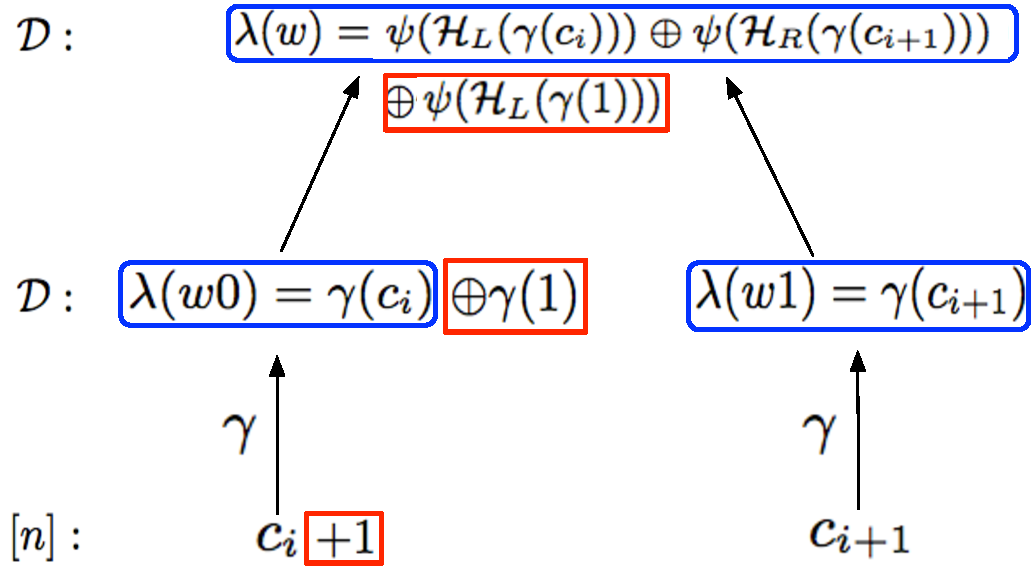
\includegraphics[scale = 0.4]{fig/update_illustrate.pdf}
\caption{Update of labels. At the leaf nodes $w0$ and $w1$, frequency values $c_{i}$ and $c_{i+1}$ are stored respectively. The labels of $w0$ and $w1$ are therefore $\gamma(c_{i})$ and $\gamma(c_{i+1})$. By Definition~\ref{main_expression}, the label of their parent node $w$ is $\psi ( {\cal H}_{L} ( \gamma (c_{i})))  \oplus \psi ( {\cal H}_{R} ( \gamma (c_{i+1}) ))$. Now, assume frequency value stored at leaf $w0$ is updated to $c_{i}+1$. The label of $w0$ can simply be updated by an $\oplus$ operation with $\gamma(1)$. Similarly, the label of $w$ is updated by an $\oplus$ operation with $\psi ( {\cal H}_{L} ( \gamma (1) ))$.}\label{label_update}
\end{figure}

\begin{defn}[Labeling function]\label{main_expression}
Let $T_\mathcal{C}$ be a structured binary tree, where $\mathcal{C}=[c_0, c_1, \ldots,c_{M-1}]$. For every node $w\in T_{\mathcal{C}}$, we define its labeling as $\lambda(w) ={\sum_{v\in \mathsf{range}(w)}} \mathcal{L}_w(v) \in {\mathcal{D}}$.
\end{defn}

E.g., Figure~\ref{label_update} illustrates a simple example of the labeling function. At the leaf level of a generalized hash tree, frequency values $c_{i}$ and $c_{i+1}$ are stored at leaf node $w0$ and $w1$. Hence, the labels of $w0$ and $w1$ are $\lambda(w0) = \gamma(c_{i})$ and $\lambda(w1) = \gamma(c_{i+1})$. By Definition~\ref{main_expression}, the label of their parent node $w$ should be the summation over ${\mathcal{D}}$ of the partial labels of $w$ with respect to $w0$ and $w1$. Hence, $\lambda(w) = \psi ( {\cal H}_{L} ( \gamma (c_{i})))  \oplus \psi ( {\cal H}_{R} ( \gamma (c_{i+1}) ))$.

%{\bf Constraint.} In a legitimate generalized hash tree, the labeling of each node must be in domain $\mathcal{D}$. Hence, our choices of hash function, projection function and $\gamma$ need to guarantee 
%\begin{equation}\label{constraint}
%\sum_{v\in \mathsf{range}(w)} \mathcal{L}_w(v) \in \mathcal{D} \text{,  for every node } w\in T_{\mathcal{C}}. 
%\end{equation}
%In~\cite{Papa}, function $\gamma$ is defined by $\gamma(c_{v}) = c_{v} \cdot {\bf 1}$. This setup, together with the projection function choice, ensures that every node labeling has a legitimate value in the domain.


%We now prove the following two important lemmas that we are going to use to prove the final result (generalized hash tree):

\begin{lemma}\label{property-2}
Let $T_\mathcal{C}$ be a structured binary tree. Let $h, \phi, \lambda$ be the hash function, projection function and labeling function described above. Then, $\phi(\lambda(w)) = h(\lambda(w{0}), \lambda(w{1}))$, where $w$ is any internal node of $T_\mathcal{C}$ and $w{0}, w{1}$ are two children of $w$.
\end{lemma}
\begin{proof}
\begingroup\makeatletter\def\f@size{7.5}\check@mathfonts
\def\maketag@@@#1{\hbox{\m@th\large\normalfont#1}}%
\begin{align*}
&\phi(\lambda(w))=\phi\left(\sum_{v\in \mathsf{range}(w)} \mathcal{L}_w(v)\in {\mathcal{D}} \right) 
\nonumber \text{\ \ (Def.~\ref{main_expression})}\\
&={\sum_{v\in \mathsf{range}(w0)} \phi\left(\mathcal{L}_w(v)\right)} \otimes \sum_{v\in \mathsf{range}(w1)}\phi\left(\mathcal{L}_w(v)\right) 
\nonumber \text{\ \ (Def.~\ref{hashfunction})}\\
&=\sum_{v\in \mathsf{range}(w0)}\phi\left(g_{w-v}(\gamma (c_v))\right) \otimes \sum_{v\in \mathsf{range}(w1)}\phi\left(g_{w-v}(\gamma(c_v))\right) 
\nonumber \text{\ \ (Def.~\ref{weight_of_a_node})}\\
%&=&\sum_{v\in \mathsf{range}(w0)}\phi\left(g_0(g_{w0-v}(\gamma(c_v)))\right)+\sum_{v\in \mathsf{range}(w1)}\phi\left(g_1(g_{w1-v}(\gamma(c_v)))\right)
%\nonumber \text{\ \ (Def.~\ref{compose_def})}\\
&=\sum_{v\in \mathsf{range}(w0)}\phi\left(g_0(\mathcal{L}_{w0}(v))\right) \otimes \sum_{v\in \mathsf{range}(w1)}\phi\left(g_1(\mathcal{L}_{w1}(v))\right) 
\nonumber \text{\ \ (Def.~\ref{weight_of_a_node})}\\
&=\sum_{v\in \mathsf{range}(w0)}\phi\left(\psi( {\bf {\cal H}_{L}} \cdot \mathcal{L}_{w0}(v))\right) \\
& \quad \quad \otimes \sum_{v\in \mathsf{range}(w1)}\phi \left(\psi({\bf {\cal H}_{R}} \cdot\mathcal{L}_{w1}(v))\right) 
\nonumber \text{\ \ (Def.~\ref{compose_def})}\\
&=\sum_{v\in \mathsf{range}(w0)} {\bf {\cal H}_{L}} \cdot\mathcal{L}_{w0}(v)
 \otimes \sum_{v\in \mathsf{range}(w1)}{\bf {\cal H}_{R}}\cdot\mathcal{L}_{w1}(v) 
\nonumber \text{\ \ (Cor.~\ref{phipsi})}\\
&={\bf {\cal H}_{L}} (\lambda(w0)) \otimes {\bf {\cal H}_{R}} (\lambda(w1)  ) =h(\lambda(w0), \lambda(w1)).
\nonumber \text{\ \ (Def.~\ref{main_expression})} 
\end{align*}\endgroup
\end{proof}
%\babis{you might want to put reference to definitions and relative corollaries back in}
\begin{theorem}\label{final_thm}
Let $T_\mathcal{C}$ be a structured binary tree. Then, $(T_\mathcal{C},\lambda,$\\
$f,h)$ is a generalized hash tree, where $h, \phi, \lambda$ are the hash function, projection function and labeling function described above. .
\end{theorem}
\begin{proof}
It follows from Lemma~\ref{property-2} and by Definition~\ref{def_generalized}. 
\end{proof}

\subsection{Efficient updates of the labels}
The output $\lambda(v)$ of the labeling function applied to node $v$ can be updated very efficiently whenever the leaf changes. We first introduce the following definition.
\begin{defn}[Unit update]\label{delta}
For any internal node $w \in T_{\mathcal{C}}$ and any leaf node $v \in T_{\mathcal{C}}$, let the unit update of $w$ in terms of $v$ be $\delta_w(v) = g_{\epsilon - v_{i}}(\gamma(1))$.
\end{defn}
Each occurrence of an element $i$ contributes $\delta_w(i)=g_{w - v_{i}}(\gamma(1))$ on the internal node $w$. Adding (or removing) an element $i$ is equivalent to adding (or subtracting) $\delta_w(i)$ to (from) $\lambda(w)$. It is important to note that computing a unit update, as well as a partial label, only requires $O(\log M)$ recursive calls of hash function $h$. 

Figure~\ref{label_update} shows how to update the corresponding labels when the value stored at leaf node $w0$ increments by $1$. For a more concrete example, let $\lambda(\epsilon)$ be the label of the root of a generalized hash tree $(T_{\mathcal{C}},\lambda,\phi,h)$ with eight leaves $\{v_{0},v_{1},\ldots,v_{7}\}$ where $c_3=2$, $c_4=c_6=c_7=1$ and $c_0=c_1=c_2=c_5=0$. By Corollary~\ref{prune}, the root label $\lambda(\epsilon) = \sum_{v\in \mathsf{range}(\epsilon)} \mathcal{L}_w(v)\in {\mathcal{D}}$ can be expressed as $ \mathcal{L}_\epsilon(v_{2})+\mathcal{L}_\epsilon(v_{4})+\mathcal{L}_\epsilon(v_{6})+\mathcal{L}_\epsilon(v_{7})$. Adding (or removing) an element $i$ is equivalent to adding (or subtracting) $\delta_\epsilon(i)$ to (from) $\lambda(\epsilon)$, which only takes $O(\log M)$ calls of $h$.
\subsection{SADS construction}\label{streaming_dictionary}
Let $T_{\mathcal{C}}$ be a structured binary tree with $M$ leaves corresponding to the universe. Let $(T_{\mathcal{C}},\lambda,\phi,h)$ denote the generalized hash tree of interest as described above. To store the generalized hash tree, we store only the labels that are defined on the paths from non-zero leaves to the root (all other labels are zero). This requires space proportional to $O(\nu \log M)$, where $\nu$ is the number of distinct element appearing in the stream. Figure~\ref{algorithms_sads} presents the 6 algorithms of our abstract SADS scheme. 


{\bf Range search queries.}
The abstract SADS inherits the query expressiveness from the PSTY work~\cite{DBLP:conf/eurocrypt/PapamanthouSTY13}. It supports the range search queries by the same algorithm.

 The proof for a range search query $[x,y]$ simply contains the two proofs $\Pi(x)$ and $\Pi(y)$ as output by algorithms $\mathsf{query}(x,D_h,\mathsf{auth}$\\
 $(D_h),\mathsf{pk})$ and $\mathsf{query}(y,D_h,\mathsf{auth}(D_h),\mathsf{pk})$ respectively from Figure~\ref{algorithms_sads}. It also contains the frequencies $\mathcal{C}_{xy}=\{c_{a_1},c_{a_2},\ldots,c_{a_s}\}$ of the reported range as an answer. Let now $\mathcal{R}_{xy}=\{a_1,a_2,\ldots,a_s\}$ denote the respective reported range that corresponds to $\mathcal{C}_{xy}$.

%\frame box[2.8][l]{{\bf Algorithm} $\mathsf{pk}\leftarrow\mathsf{genkey}(1^\lambda,n)$: } \par

\begin{figure*}[ht!]
{
\centering
\framebox{\parbox{0.99\textwidth}{
\paragraph{\textbf{Algorithm}  $\mathsf{pk}\leftarrow\mathsf{genkey}(1^\lambda,n)$} On input the security parameter $\lambda$ and a bound $n$ on the size of the stream, set $\mathsf{pk}=\{\vc{L},\vc{R},{\cal U}\}$, where ${\cal U}$ is a universe such that $|{\cal U}|=M$ and $\vc{L},\vc{R}$ specify the hash function.
}}} 
%\newline\newline
{\centering
\framebox{\parbox{0.99\textwidth}{
\paragraph{\textbf{Algorithm}  $\{\mathsf{auth}(D_0),d_0\}\leftarrow\mathsf{initialize}(D_0,\mathsf{pk})$} Let $D_0$ be a structured binary tree $T_\mathcal{C}$ where $c_i=0$ ($i=0,\ldots,M-1$). The algorithm outputs the generalized hash tree $(T_{\mathcal{C}},\lambda,\phi,h)$ as $\mathsf{auth}(D_0)$, where $\lambda(v)={\bf 0_{\mathcal{D}}}$ for all nodes $v$ in $T_{\mathcal{C}}$. Also it outputs $d_0={\bf 0_{\mathcal{D}}}$. 
}}}
{\centering
\framebox{\parbox{0.99\textwidth}{
\paragraph{\textbf{Algorithm}  $d_{h+1}\leftarrow\mathsf{updateVerifier}(x,d_h,\mathsf{pk})$} Let $x\in {\cal U}$ be the current element of the stream. The algorithm updates the local state by setting $d_{h+1}=d_h \oplus \delta_{\epsilon}(x)$, where $\epsilon$ is the root of $T_{\mathcal{C}}$ and $\delta_{\epsilon}(x)$ is defined in Definition~\ref{delta}.%and $\vc{1}$ is the unit vector of $k$ entries.
}}}
{\centering
\framebox{\parbox{0.99\textwidth}{
\paragraph{\textbf{Algorithm} $\{D_{h+1},\mathsf{auth}(D_{h+1})\}\leftarrow\mathsf{updateProver}(x,D_h,\mathsf{auth}(D_h),\mathsf{pk})$}
Let $x\in {\cal U}$ be the current element of the stream. The algorithm sets $c_x=c_x+1$, outputting the updated tree $T_{\mathcal{C}}$. Let $v_{\ell},\ldots,v_1$ be the path in $T_{\mathcal{C}}$ from node $v_{\ell}$ ($v_{\ell}$ stores $c_x$) to the child $v_1$ of the root $\epsilon$ of $T_{\mathcal{C}}$. Set
\begin{equation}\label{structure_update}
\lambda(v_i)=\lambda(v_i) \oplus \delta_{v_{i}}(x) \text{\ for $i=\ell,\ell-1,\ldots,1$}\,,
\end{equation}
where $\delta_{v_{i}}(x)$ is defined in Definition~\ref{delta}. The new authenticated data structure $\mathsf{auth}(D_{h+1})$ is the new generalized hash tree with the updated labels as computed in Equation~\ref{structure_update}.
}}}
{\centering
\framebox{\parbox{0.99\textwidth}{
\paragraph{\textbf{Algorithm} $\{\alpha(q),\Pi(q)\}\leftarrow\mathsf{query}(q,D_h,\mathsf{auth}(D_h),\mathsf{pk})$} Let $q$ be a frequency query for element $x\in {\cal U}$. Set $\alpha(q)=c_x$ (note that if $c_x=0$, $x$ is not contained in the collection). Let $v_{\ell},\ldots,v_1$ be the path in the structured binary tree $T_{\mathcal{C}}$ from node $v_{\ell}$ ($v_{\ell}$ stores the value $c_x$) to the child $v_1$ of the root $\epsilon$ of $T_{\mathcal{C}}$. Let also $w_{\ell},\ldots,w_1$ be the \emph{sibling nodes} of $v_{\ell},\ldots,v_1$. Proof $\Pi(q)$ contains the ordered sequence of the pairs of labels belonging to the tree path from leaf $v_\ell$ to the root $\epsilon$ of the tree, i.e., the pairs $\{(\lambda(v_{\ell}),\lambda(w_{\ell})),(\lambda(v_{\ell-1}),\lambda(w_{\ell-1})),\ldots,(\lambda(v_{1}),\lambda(w_{1}))\}$.
}}}
{\centering
\framebox{\parbox{0.99\textwidth}{
\paragraph{\textbf{Algorithm} $\{{\tt{1}},{\tt{0}}\}\leftarrow
  \mathsf{verify}(q,\alpha(q),\Pi(q),d_h,\mathsf{pk})$} Let $q$ be a frequency query for element $x\in {\cal U}$. Parse $\Pi(q)$ as $$\{(\lambda(v_{\ell}),\lambda(w_{\ell})),\ldots,(\lambda(v_{1}),\lambda(w_{1}))\}$$ and $\alpha(q)$ as $c_x$. 

If $\lambda(v_{\ell})\ne \gamma(c_x) $ or $\lambda(v_{\ell}),\lambda(w_{\ell}) \notin {\mathcal{D}}$, output ${\tt{0}}$. Compute values $y_{\ell-1},y_{\ell-2},\ldots,y_0$ as $y_i=h(\lambda(v_{i+1}), \lambda(w_{i+1}))$ (if $v_{i+1}$ is $v_{i}$'s left child) or $y_i=h(\lambda(v_{i+1}),\lambda(w_{i+1}))$ (if $v_{i+1}$ is $v_{i}$'s right child). For $i=\ell-1,\ldots,1$, if $\phi(\lambda(v_i))\ne y_i$ \textbf{or} $\lambda(v_i),\lambda(w_i)\notin {\mathcal{D}}$ output ${\tt{0}}$. If $\phi(d_h)\ne y_0$, output ${\tt{0}}$. Output ${\tt{1}}$.
}}}
%\newline
\footnotetext{If $v_{i+1}$ is $v_{i}$'s right child, we set $y_{i}=\vc{R}\cdot\lambda(v_{i+1})+\vc{L}\cdot\lambda(w_{i+1})$.}
\caption{\label{algorithms_sads}Algorithms of the abstract SADS for verifying frequency queries.}
\end{figure*}


For verification, the proofs $\Pi(x)$ and $\Pi(y)$ are verified first by using algorithm $\mathsf{verify}$ from Figure~\ref{algorithms_sads}. If this verification is successful, perform the following test (else reject): If for all labels $\lambda(v)\in \Pi(x) \cup \Pi(y)$ such that $\mathsf{range}(v)\cap\mathcal{R}_{xy}$ is not empty, the following relation (as in Definition~\ref{main_expression}) 
\begin{equation}\label{eq:check_efficiency}
\lambda(v) =\sum_{i\in \mathsf{range}(v)\cap\mathcal{R}_{xy}} \mathcal{L}_v(i)
\end{equation}
is true, output $\tt{1}$ (i.e., accept), else output $\tt{0}$ (i.e., reject).
The above relation ensures that all the range (with the correct frequencies) has been reported, or otherwise, the adversary could find a collision. The above technique can be also used for verifying successor queries, where the reported range is empty.

\subsection{PSTY instantiation of our abstract SADS}\label{instantiation}
We show the PSTY scheme~\cite{DBLP:conf/eurocrypt/PapamanthouSTY13} is an instantiation of our abstract SADS. Recall our SADS is built upon a generalized hash tree $(T,\lambda,\phi,h_{old})$, where $h_{old}$ is a collision resistant hash function, $\phi$ is a projection function and $\lambda$ is a labeling function. In particular, the labeling function $\lambda$ is determined by the hash function $h_{old}$, the $\gamma$ function and the inverse projection function $\psi$. We next study all four components of the PSTY scheme~\cite{DBLP:conf/eurocrypt/PapamanthouSTY13}.

{\bf Hash function.} 
The hash function $h_{old}$ uses ${\mathcal{D}}= \mathbb{Z}_n^{t}$ and ${\mathcal{R}} = \mathbb{Z}_q^{\nu}$ as its domain and range. The operation $\oplus$ of ${\mathcal{D}}$ is mod $n$ addition, and the operation $\otimes$ of ${\mathcal{R}}$ is mod $q$ addition. 
Specificially, $h_{old}$ is defined as: 
\begin{enumerate}
\item $h_{old} ({\bf x, y})= {\bf {\cal H}_{L}(x)}  + {\bf {\cal H}_{R}(y)}$ mod q;
\item ${\bf {\cal H}_{A}(x)} = {\bf A \cdot x}$ mod q, where $\bf A= L, R$ is a randomly picked matrix from $\mathbb{Z}_q^{\nu \times t}$.
\end{enumerate}
${\bf {\cal H}_{A}}$ is collision resistant based on the hardness assumption of the small integer solution problem $\mathsf{SIS}_{q, t,\beta}$~\cite{DBLP:journals/siamcomp/MicciancioR07}. Here, $q$ is a large prime, $t=\nu \lceil \log q \rceil$, $\beta$ is set to $n\sqrt{2t}$.

First, we show $h_{old}$ is collision resistant. Assume there exist $\bf x_{\delta}, y_{\delta} \neq 0_{\mathcal{D}}$ such that $\bf {\cal H}_{L}(x_{\delta}) + {\cal H}_{R}(y_{\delta})= {\bf 0}_{\mathcal{R}}$ with non-negligible probability. This would give a solution to $\mathsf{SIS}_{q, 2t,\beta}$ with the matrix be $[L,\, R]$ randomly chosen from $\mathbb{Z}_q^{\nu \times 2t}$. 


%Let $q$ be a large enough prime, $t=\lambda \lceil \log q \rceil$ and $\beta=n\sqrt{2t}$. The hash function $h_{old}$ uses ${\mathcal{D}}= \mathbb{Z}_n^{t}$ and ${\mathcal{R}} = \mathbb{Z}_q^{\lambda}$. The operation $\oplus$ of ${\mathcal{D}}$ is mod $n$ addition, and the operation $\otimes$ of ${\mathcal{R}}$ is mod $q$ addition. 
%Specificially, $h_{old}$ is defined as: 
%\begin{enumerate}
%\item $h_{old} ({\bf x, y})= {\bf {\cal H}_{L}(x)}  + {\bf {\cal H}_{R}(y)}$ mod q;
%\item ${\bf {\cal H}_{A}(x)} = {\bf A \cdot x}$ mod q, where $\bf A= L, R$ is a randomly picked matrix from $\mathbb{Z}_q^{\lambda \times t}$.
%\end{enumerate}
%First, ${\bf {\cal H}_{A}}$ is collision resistant based on the hardness assumption of the small integer solution problem $\mathsf{SIS}_{q, t,\beta}$~\cite{DBLP:journals/siamcomp/MicciancioR07}. Assume there exist $\bf x_{\delta}, y_{\delta} \neq 0_{\mathcal{D}}$ such that $\bf {\cal H}_{L}(x_{\delta}) + {\cal H}_{R}(y_{\delta})= {\bf 0}_{\mathcal{R}}$ with non-negligible probability. But this would give a solution to $\mathsf{SIS}_{q, 2t,\beta}$ with the matrix be $[L,\, R]$ in $\mathbb{Z}_q^{\lambda \times 2t}$. Hence, $h_{old}$ is collision resistant.

Second, given ${\bf x, y} \in {\mathcal{D}}$ such that ${\bf x + y} \in {\mathcal{D}}$, it is obvious that $${\bf {\cal H}_{A}(x \oplus y)} = {\bf {\cal H}_{A}(x + y)} = {\bf A \cdot x} + {\bf A \cdot y} \text{  mod q}.$$The labeling function below ensures that for any two labels ${\bf x, y} \in {\mathcal{D}}$ in the generalized hash tree, ${\bf x + y} \in {\mathcal{D}}$ holds. 

From the above two arguments, $h_{old}$ meets the characterization of Definition~\ref{hashfunction}.

{\bf Projection function.}
The projection function $\phi: \mathbb{Z}_n^{t} \rightarrow \mathbb{Z}_q^\nu$ \emph{parses} the input vector $\vc{x}$ as a radix-2 representation (i.e., a base-2 representation but not necessarily of binary coefficients) and converts it to the respective vector in $\mathbb{Z}_q^\nu$. 

On input a vector $\vc{x}\in \mathbb{Z}_n^{t}$, where $\tau = \lceil \log q \rceil$ and $t=\nu \cdot \tau$, output a vector $\vc{y} = \phi(\vc{x})$ of $\nu$ entries such that each $\vc{y}_i$ ($i=0,\ldots,\nu-1$) is the number in $\mathbb{Z}_q$ represented by the radix-2 representation $[\vc{x}_{i\tau},\vc{x}_{i\tau+1},\ldots,\vc{x}_{(i+1)\tau-1}]^{\mathsf{T}}$, namely $$\vc{y}_i=\sum_{j=0}^{\tau-1}\vc{x}_{i\tau +j}2^j\mod q\,,\text{ for $i=0,\ldots,\nu-1$}\,.$$

It is easy to check that $\phi$ here forms a surjective homomorphism from $\mathbb{Z}_n^{t}$ to $\mathbb{Z}_q^\nu$. 

{\bf Inverse projection function.}
The inverse projection function $\psi: \mathbb{Z}_q^\nu \rightarrow \mathbb{Z}_n^{t}$ is simply the binary representation of vectors. For example, if $\nu=2$, $q=8$ and $\vc{a}=[6,3]^{\mathsf{T}}\in \mathbb{Z}_8^2$, then $\psi (\vc{a})=[1,1,0,0,1,1]^{\mathsf{T}}$, since $\psi(6)=[1,1,0]^{\mathsf{T}}$ and  $\psi(3)=[0,1,1]^{\mathsf{T}}$. Obviously, $\psi$ here satisfies Definition~\ref{inverseprojection}.

{\bf $\gamma$ function. }
The gamma function $\gamma: [n] \rightarrow \mathbb{Z}_n^{t}$ is defined as:
\begin{equation}\label{gamma1}
\gamma(c_{v}) = c_{v} \cdot {\bf 1}, 
\end{equation}
where $\vc{\emph{1}}= [1, 1, \ldots, 1]^{\mathsf{T}} \in \mathbb{Z}_n^{t}$. Clearly, $\gamma(c_{v1}+c_{v2}) = \gamma(c_{v1}) + \gamma(c_{v2})$ mod n, given $c_{v1}+c_{v2} \in [n]$. 

Let $T_{C}= (T, \lambda, \phi, h_{old})$ be the generalized hash tree as described above. For any node $w \in T_{C}$, by Definition~\ref{main_expression} we have its label $\lambda(w) ={\sum_{v\in \mathsf{range}(w)}} \mathcal{L}_w(v) \in {\mathcal{D}}$ . Since the entries of each partial label $\mathcal{L}_w(v) = c_{v} \cdot \{0,1\}^{t}$ and $\sum_{i=0}^{M-1}c_i\le n$, we know $\lambda(w)\in \mathbb{Z}_{n}^t$. It follows that for any two labels ${\bf x, y} \in T_{C}$, ${\bf x+y}  \in \mathbb{Z}_{n}^t$ is also true. Therefore, $T_{C}$, as it is described in PSTY~\cite{DBLP:conf/eurocrypt/PapamanthouSTY13}, is an instance of the abstract SADS.

In the following sections, we show how to build an improved instantiation of the abstract SADS by employing a better hash function. The choices of the {\it projection function}, the {\it inverse projection function} and {\it $\gamma$ function} {\bf remain the same}.
%We now give our final result stating the formal security guarantee of our algorithms, along with their detailed asymptotic performance. The correctness of our scheme follows easily by inspecting the algorithms, therefore its proof is omitted. The security proof and the proof of asymptotic performance are in the Appendix.
%\begin{theorem}[Streaming authenticated frequency with range search]\label{main_theorem_lattice}
%Let $k$ be the security parameter, $n=\mathsf{poly}(k)$ be an upper bound on the size of a stream containing elements from an ordered universe $\mathcal{U}$ of size $M$, $\{q,\mu,\beta\}\leftarrow {\sf parameters}(1^k,n)$ and $\nu$ be the number of unique elements that have appeared in the stream. There exists a streaming authenticated data structure scheme for one-dimensional frequency queries and one-dimensional range queries (outputting the respective frequencies) such that: \textbf{(a)} It is correct according to Definition~\ref{sound_def} and secure according to Definition~\ref{sec_def_general} and assuming hardness of $\mathsf{SIS}_{q,\mu,\beta}$ (Assumption~\ref{assume_sis}); \textbf{(b)} Algorithms $\mathsf{updateVerifier}$ and $\mathsf{updateProver}$ run in $O(\log M\log^2 n)$ time; \textbf{(c)} Algorithm $\mathsf{query}$ (both for frequency and range search queries) runs in $O(\log M\log n)$ time, outputting a proof of size $O(\log M\log n)$; \textbf{(d)} A frequency query can be verified in $O(\log M\log ^2 n)$ time and a range search query can be verified in $O(s\log M\log ^2 n)$ time, where $s$ is the size of the output range; \textbf{(e)} The space required at the verifier is $O(\log n)$ and the space required at the prover is $O(\nu\log M\log n)$. 
%\end{theorem}

%Our algorithms can be extended to two (or multiple) dimensions by leveraging existing methods for multidimensional range queries~\cite{DBLP:journals/algorithmica/MartelNDGKS04}, carefully adjusted in our framework. Due to space limitations, we defer such extensions to the full version of our paper.











\vfill\eject\section{New Hash Function based on Generalized Knapsack Problem}\label{gck}
In the implementation of our SADS, we found the hash function $h_{old}$ in PSTY~\cite{DBLP:conf/eurocrypt/PapamanthouSTY13} computationally costly both in terms of running time and key size.  
We study both the algebraic and the security properties of the Generalized Compact Knapsack problem (GCK), and take a subclass of GCK hash functions to instantiate our SADS.

{\bf Preliminaries.} We give a brief preliminary review on rings and ideals. Please refer to~\cite{algebrabook} for a comprehensive study. Let $\mathbb{Z}[x]$ and $\mathbb{R}[x]$ be the set of polynomials with integers and real coefficients. A polynomial is {\it monic} if the coefficient of the highest power is $1$. A polynomial is {\it irreducible} if it cannot be represented as a product of lower degree polynomials. Each polynomial corresponds to a vector of its coefficients. E.g., we can represent polynomial $a_{0}+\ldots+a_{k-1}x^{k-1}$ simply as $(a_{0},\ldots,a_{k-1})$. We define the $l_{p}$ norm $|g(x)|_{p}$ of a polynomial $g(x)$ as the norm of the corresponding vector.

Let $R$ be a ring. An {\it ideal} $I$ of $R$ is an additive subgroup of $R$ closed under multiplication by arbitrary $g \in R$. For any ring $f \in R$, $\langle f \rangle$ denotes the set of all multiples of $f$. The quotient $R/I$ is the set of all equivalence classes $(g+I)$ of $R$ modulo $I$.

Let $\mathcal{R}= \mathbb{Z}[x]/\langle f \rangle$ where $f$ is monic and irreducible. When $f$ is monic and of degree $k$, every equivalence calss $(g+\langle f \rangle) \in \mathbb{Z}[x]/\langle f \rangle$ has a unique representative $g^{'} \in (g+\langle f \rangle) $ of degree less than $k$. We define the norm $|(g+\langle f \rangle)|_{f}$ over ring $ \mathbb{Z}[x]/\langle f \rangle$ as $|g$ mod $f|_{\infty}$. As short hand, we write $|g|_{f}$ instead of $|(g+\langle f \rangle)|_{f}$. 

In this paper, we focus on the ring $\mathcal{R}= \mathbb{Z}_{p}[\alpha]/(\alpha^{k}+1)$, where $k-1$ is the highest degree of an arbitrary $g \in \mathcal{R}$ and $p$ is a prime. 
\subsection{Generalized Compact Knapsack Problem}
We begin with a brief review of the Generalized Compact Knapsack problem. Lyubasevsky et al propose an efficient SWIFFT hash that is provably collision-resistant~\cite{swifft}. Finding a collision on the average with any noticeable probability is at least as hard as solving worst case problems for cyclic lattices. The SWIFFT function has a simple algebraic expression over the ring $\mathcal{R}= \mathbb{Z}_{p}[\alpha]/(\alpha^{k}+1)$. A particular function in the family is specified by $m$ fixed ${{\bf a}_{1},\ldots, {\bf a}_{m}} \in \mathcal{R}$. The function corresponds to the following expression over the ring $\mathcal{R}$:
\[ \Sigma_{i=1}^{m} ({\bf a}_{i} \cdot {\bf x}_{i})   \,\, \in \mathcal{R},\]
where ${\bf x}_{1} ,\ldots, {\bf x}_{m} \in \mathcal{R}$ are polynomials with binary coefficients, and corresponding to the input of length $k \cdot m$.

The above formula is a special instance of generalized compact knapsack problem proposed in~\cite{GCK}. 
\begin{defn}{\bf (GCK problem).}
Given $m$ random elements ${\bf a}_{1},\ldots, {\bf a}_{m} \in \mathcal{R}$ for some ring, and a target ${\bf t} \in \mathcal{R}$, find elements ${\bf x}_{1}, \ldots, {\bf x}_{m} \in \mathcal{I}$ such that $\Sigma_{i=1}^{m} {\bf a}_{i}\cdot {\bf x}_{i} ={\bf t}$, where $\mathcal{I}$ is some given subset of $\mathcal{R}$.
\end{defn}

Lyubashevsky and Micciancio prove that for appropriate choices of $\mathcal{R}$ and $\mathcal{I}$, finding collisions in such hash functions is at least as hard as solving worst case hard problems on ideal lattices~\cite{GCK}. We present the constraints on $\mathcal{R}$ and $\mathcal{I}$ to make $\cal H$ collision-resistant~\cite{GCK}.
\begin{enumerate}
\item Ring $\mathcal{R}= \mathbb{Z}[\alpha]_{p}/\langle f \rangle$, where $f \in \mathbb{Z}[\alpha]$ is irreducible, monic polynomial of degree $n$ with expansion factor $EF(f,3) \leq \varepsilon$. The definition of expansion factor is as the following.
\[ EF(f,q) = \max_{g \in \mathbb{Z}[\alpha], deg(g) \leq q(deg(f)-1)} |g|_{f}/|g|_{\infty}\] \label{CRcon1}
\item $\mathcal{I}=\{g \in \mathcal{R}: |g|_{f} \leq d\}$, where $d$ is some positive integer. \label{CRcon2}
\item It is required that $m > \log p / \log 2d$ and $p > 2 \varepsilon d mk^{1.5} \log k$.\label{CRcon3}
\end{enumerate}

\subsection{New Hash Function}\label{new_hash}
We focus on the following GCK hash function family $\{{\cal H}_{\bf A}\}: \mathcal{D} \rightarrow \mathcal{R}$, where $\mathcal{D} = \mathcal{I}^{m} = \mathbb{Z}_{n}^{k\cdot m}$ and $\mathcal{R}= \mathbb{Z}[\alpha]_{p}/\langle \alpha^{k}+1 \rangle$. 

Given input $X=[{\bf x}_{1}, {\bf x}_{2}, \ldots, {\bf x}_{m}] \in \mathcal{D}$, 
\begin{equation}\label{product}
 {\cal H}_{\bf A}(X) = \Sigma_{i=1}^{m} ({\bf a_{i} \cdot x_{i}})   \,\, \in \mathcal{R},
\end{equation}
where $A=[{\bf a}_{1},\ldots,{\bf a}_{m} ]$ and each ${\bf a}_{i}\in \mathcal{R}$.

We construct a subclass of collision-resistant GCK hash functions from the above function family by careful parameter selection. First, since $EF(f,3) \leq 3$ is proved for $f=\alpha^{k}+1$ in~\cite{GCK}, $\varepsilon$ in the constraints above can be set to $3$. By picking a large enough prime $p$ such that $p/\log p > 6nk^{1.5} \log k$ and setting $m = \lceil \log p \rceil$, it is easy to check that conditions~\ref{CRcon1}~\ref{CRcon2}~\ref{CRcon3} for ${\cal H}_{\bf A}$ to be collision resistant are all met. %\babis{please put numbers and refer to equations above}
%\babis{change $h_{old}$ to $h_{old}$ and $h_n$ to $h_{new}$}
Second, we make ${\cal H}_{\bf A}$ achieve the desired level of security against the best known attack algorithms by additional constraints. Figure~\ref{config_alg} shows the algorithm of parameter configuration for our GCK hash function. In particular, constraints~\ref{constraint_1} and~\ref{constraint_4} make ${\cal H}_{\bf A}$ theoretically collision resistant; constraints~\ref{gba_constraint} and~\ref{lattice_constraint} ensure ${\cal H}_{\bf A}$ reaches the level of security $\lambda$ against the best known algorithms of the {\it generalized birthday attack}~\cite{wagner02} and the {\it lattice attack}~\cite{lattice} respectively. We study the cryptanalysis of ${\cal H}_{\bf A}$ in section~\ref{attacks}.
\begin{figure}[h!]
{\centering
\framebox{\parbox{0.46\textwidth}{
\paragraph{\textbf{Algorithm}  $\{k, p, m\} \leftarrow  (n, \lambda) $} 
Let $k$ be a power of $2$ and $p$ be a prime. Find the smallest $k$ and then the smallest $p$ such that
\begin{enumerate}
\item $p/\log (p) > 6nk^{1.5} \log k$;\label{constraint_1}
\item $2^{\lfloor{\log m} \rfloor} p^{k/(1+\lfloor{\log m} \rfloor)} \geq 2^{\lambda}$;\label{gba_constraint}
\item $n\sqrt{km} < 2^{2\sqrt{k \log p \log \delta}}$;\label{lattice_constraint}
\item $m = \lceil \log (p) \rceil$.\label{constraint_4}
\end{enumerate}
}}}
\caption{\label{config_alg}Parameter configuration of our GCK hash function ${\cal H}_{\bf A}$.}
\end{figure}

% we can express it in the binary form using $m$ bits, denoted as $b_{m}(x)$. For any polynomial $g \in R$, we know in the vector form $g=(z_{1}, \ldots,z_{k}) \in [p]^{k}$ and each $z_{i} \in [p]$ can be expressed in the binary form using $m$ bits. Hence, for any $g=(z_{1}, \ldots,z_{k}) \in R$, it can be uniquely expressed in $D= \{0,1\}^{k \times m}$ as $[b_{m}(z_{1}), \ldots, b_{m}(z_{k})]^{\top}$. Consequently, the constructed ${\cal H}_{\bf A}$ here is a hash function from $D= \{0,1\}^{k \times m}$ to $R \subset D$.

%\babis{PLEASE MAKE CONSISTENT $A$ and ${\bf A}$}
We construct a new hash function for our SADS based on ${\cal H}_{\bf A}$, $h_{n}: \mathbb{Z}_{n}^{k\cdot m} \times \mathbb{Z}_{n}^{k \cdot m} \rightarrow \mathbb{Z}[\alpha]_{p}/\langle \alpha^{n}+1 \rangle$, as follows.
\begin{equation} 
h_{n}{\bf (x,y)} = {\cal H}_{L}{\bf (x)} + {\cal H}_{\mathcal{R}}{\bf (y)} \quad \mod\,\,p, 
\end{equation}
where $L, R$ are randomly chosen from $\mathbb{Z}[\alpha]_{p}^{m}/\langle \alpha^{k}+1 \rangle$. By similar arguments in section~\ref{instantiation}, $h_{n}$ belongs to the class of hash functions of the abstract SADS by Definition~\ref{hashfunction}. 

The bottleneck in terms of efficiency of the GCK hash function ${\cal H}_{\bf A}$ is computing the product of two polynomials in Equation~\ref{product}. Similar as SWIFFT~\cite{swifft}, we use FFT for computing polynomial products. Notice $\alpha^{k}+1=0$, for $\alpha=e^{j \pi i / k}$ when $j$ is odd. Hence, we only need to do $k$ evaluations at $\omega^{j}$, where $\omega= e^{\pi i / k}$ and $j=1,3,\ldots,2k-1$, to interpolate the product polynomial in $\mathcal{R}= \mathbb{Z}[\alpha]_{p}/\langle \alpha^{k}+1 \rangle$.

Notice every polynomial has a unique vector representation. In our implementation, we use a vector in $[p]^{k}$ to represent a ring in $\mathcal{R}= \mathbb{Z}[\alpha]_{p}/\langle \alpha^{k}+1 \rangle$. The algorithm of our GCK hash function is given in Figure~\ref{gck_alg}.
\begin{figure}[h!]
{\centering
\framebox{\parbox{0.46\textwidth}{
\paragraph{\textbf{Algorithm}  ${\bf z} \leftarrow  (X, A) $} 
\begin{enumerate}
\item Let input $X=[{\bf x}_{1}, \ldots, {\bf x}_{m}] \in [n]^{k\times m}$. Let ringe $\mathcal{R}=\mathbb{Z}[\alpha]_{p}/\langle \alpha^{k}+1 \rangle$. $A =[{\bf a}_{1}, \ldots, {\bf a}_{m}]$, where each ${\bf a}_{i} \in \mathcal{R}$. 
\item Precompute and store FFT$({\bf a}_{i}, \omega)$ for each ${\bf a}_{i}$, where $\omega= e^{\pi i / k}$. Let $\hat{{\bf a}_{i}}$ = FFT$({\bf a}_{i}, \omega)$.
\item For $i=1,\ldots,m$, do step (4) (5).
\item For each ${\bf x}_{i}$, compute $\hat{ {\bf x}_{i}}$ = FFT$({\bf x}_{i}, \omega)$. Compute ${\bf y}_{i} = \hat{ {\bf x}_{i}} \cdot \hat{ {\bf a}_{i}}$, where $\cdot$ refers to the inner product of two vectors. Compute $\hat{{\bf y}_{i}}=\frac{1}{k}$FFT$({\bf y}_{i}, w^{-1})$. 
\item update ${\bf z} = {\bf z}+ \hat{{\bf y}_{i}} $ mod $p$.
\end{enumerate}
}}}
\caption{\label{gck_alg}Algorithms of the our GCK hash function ${\cal H}_{\bf A}$.}
\end{figure}
For each ${\bf x}_{i}$, we run twice FFT, which requires $O(k \log k )$ operations with small constant. Hence, the total running time for our algorithm is $O(k m \log k)$ with a small constant.
 
 
 
 

%\input{newhash}
\vfill\eject\section{Security Analysis}\label{attacks}
We have shown that the GCK hash function chosen in this paper is collision-resistant. In this section, we 
study its cryptanalysis, and determine the concrete levels of security against the best known attacks. Specifically, we consider the {\it generalized birthday attacks}~\cite{wagner02} and the {\it lattice attacks}~\cite{lattice}.

As it is shown in~\cite{swifft}, the product of two polynomials ${\bf a ,x } \in \mathcal{R}$ is equivalent to the matrix product of the skew-circulant matrix of $\bf a$ with $\bf x$ in the field $ \mathbb{Z}_{p}[\alpha]$. Thus, equation~\ref{product} can be represented as the matrix product of ${\cal A} \in \mathbb{Z}_{p}[\alpha]^{k \times k\cdot m}$ with ${\bf x} \in [n]^{k \cdot m}$, where ${\cal A}$ consists of $m$ skew-circulant matrices corresponding to each ${\bf a}_{i} \in \mathcal{R}$, as shown below by Equation~\ref{represent}. This formulation is the sum of a subset of the $k \cdot m$ columns of ${\cal A}$ over the field $\mathbb{Z}_{p}[\alpha]$. Relaxing the dependencies within each skew-circulant matrix, the best known algorithm for finding collision is the same one for solving the subset sum problem~\cite{wagner02}.

\begin{equation}\label{represent}
%\[
\Sigma_{i=1}^{m} ({\bf a}_{i} \cdot {\bf x}_{i})   \,\, \in R = \begin{bmatrix} {\cal A}_{1} & {\cal A}_{2} & ... & {\cal A}_{m} \end{bmatrix} \times \left[ \begin{array}{c} x_1 \\ x_2 \\ ... \\ x_{k\cdot m} \end{array} \right]
%\]
\end{equation}

%\babis{MAKE SURE YOU USE subscripts right (not bold)}
\subsection{Generalized Birthday Attacks}
Finding a collision in our GCK hash function is equivalent to finding a nonzero ${\bf x} \in \{-n,\ldots,n\}^{k\cdot m}$ such that  ${\cal A} \cdot {\bf x =0}$ mod $p$, where {\cal A} is the $k \times k\cdot m$ matrix shown above. We provide the best known attack algorithm based on Wagner's work~\cite{wagner02}.
\begin{enumerate}
\item Divide the columns of $\cal A$ into $m$ groups, each of which consists of $k$ columns. 
\item Create a list of $(2n+1)^{k}$ vectors where each vector is a different $\{-n,\ldots,n\}$ combination of $k$ columns within the group.
\item Finding one vector from each list such that their sum is $\bf 0$ in $\mathbb{Z}_{p}[\alpha]$ is the $k$-list problem studied by Wagner~\cite{wagner02}\footnote{k-list problem consider the condition when vectors are random and independent. Relaxing the dependencies is a conservative assumption. Hence, the lower bound analysis still holds}. Wagner's algorithm has $O(2^{\lfloor{\log m} \rfloor} p^{k/(1+\lfloor{\log m} \rfloor)})$ time and space complexity. By constraint~\ref{gba_constraint} in Algorithm~\ref{config_alg}, we achieve the required level of security against the best known generalized birthday attack algorthms.
\end{enumerate}
We briefly illustrate how Wagner's algorithm works here. The first observation is solving $m$-sum problem is computational equivalent to solving a $m'<m$-sum problem. Pick one vector per list from lists $m'+1, ..., m$, and denote their sum as $\bf c$. Applying the $m'$-sum algorithm to find the solution for sum$={\bf -c}$ mod $p$ over the first $m'$ lists will solve the corresponding $m$-sum problem. In our case, the $m$-sum problem is reduced to a $k'$-sum problem, where $k^{'} =2^{\lfloor \log m \rfloor}$ is the largest power of two less than $m$.
%\babis{Please improve writing}
The algorithm follows a recursive fashion on a complete binary tree of $\lfloor \log m \rfloor$ depth. It first extends each list to size $O(p^{k/(1+\lfloor{\log m} \rfloor)} )$. Then, it constructs new lists with ${h \cdot k/(1+\lfloor{\log m} \rfloor)}$ more zero entries at internal layer of height $h$. Finally, at the root we will find the vectors that gives us $\bf 0-$sum solution. Notice that this algorithm easily applies to sum=$\bf c$ problem, where $\bf c$ is an arbitrary vector.
\subsection{Lattice Attacks}
According to the analysis in~\cite{lattice}, collisions in our GCK hash functions are vectors in the $k\cdot m$-dimensional lattice with coordinates in $\{-n,\ldots,n\}$. The Euclidean length of such vectors can at most be $n\sqrt{k\cdot m}$. However, the state of art lattice reduction algorithm cannot find non-trivial lattice vectors of which the Euclidean length is less than $2^{2\sqrt{k \log p \log \delta}}$, where $\delta=1.01$. By constraint~\ref{lattice_constraint} in Algorithm~\ref{config_alg}, the best known lattice attack algorithm cannot find collision in our GCK hash functions efficiently. 



\begin{figure*}[ht!]
\centering
\begin{minipage}[t]{.49\textwidth}
\centering
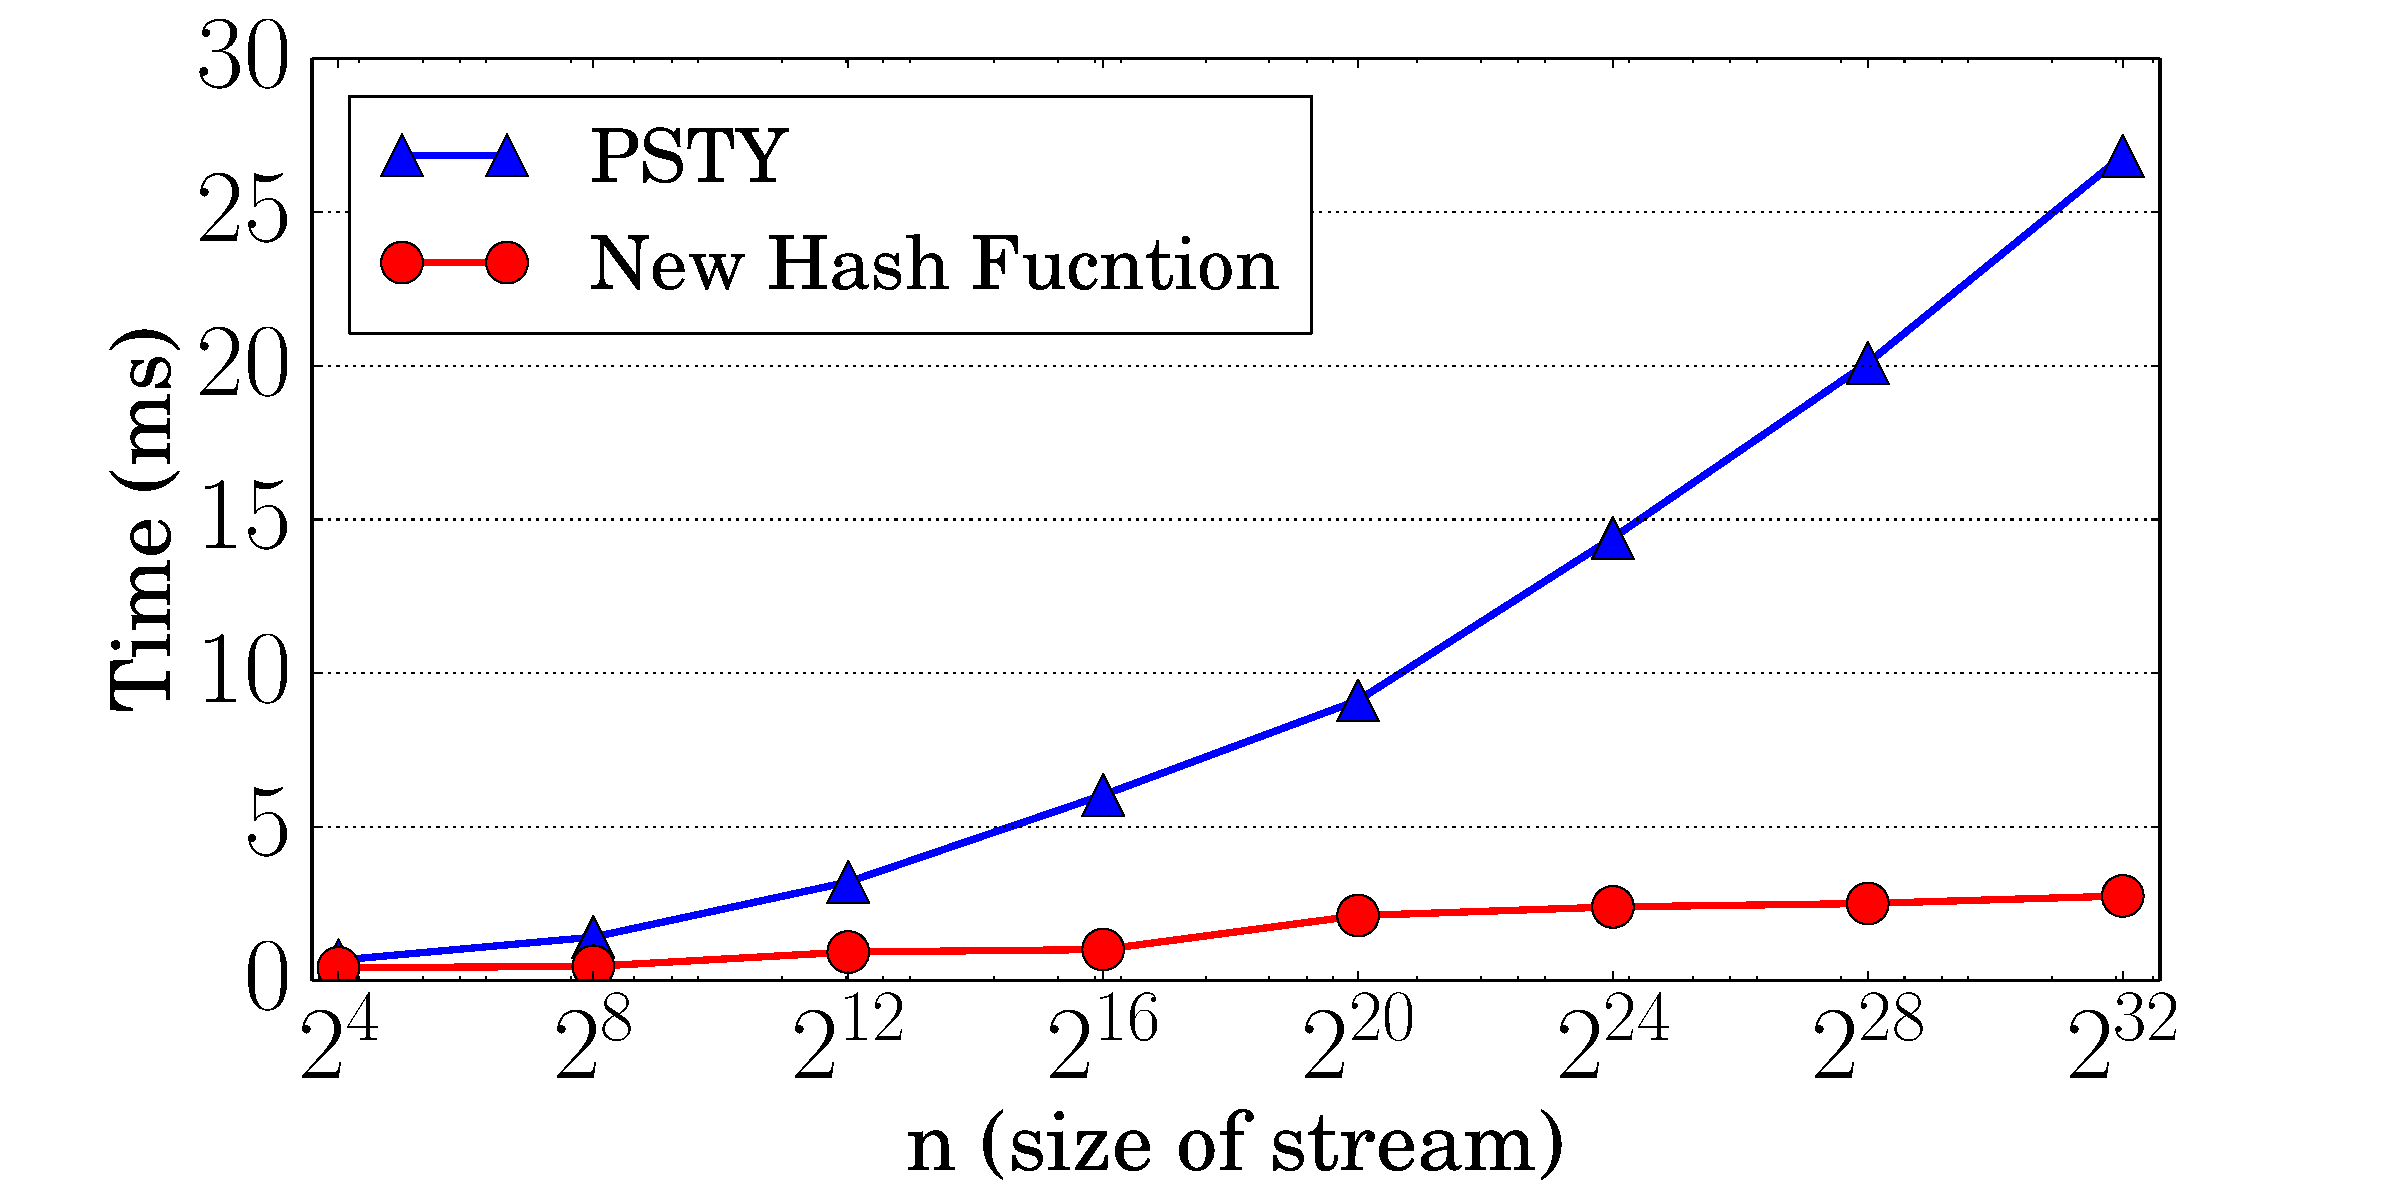
\includegraphics[scale = 0.23]{fig/hashtime.pdf}
\caption{Running time of the hash functions. In the $x$ axis, we present the size $n$ of the stream in $\log$ scale. The new hash function $h_{new}$ is $1.6\times$ faster when $n = 2^4$, and $9.8\times$ faster when $n=2^{32}$, than $h_{old}$.}\label{hashtime}
\end{minipage}\hfill
\begin{minipage}[t]{.49\textwidth}
\centering
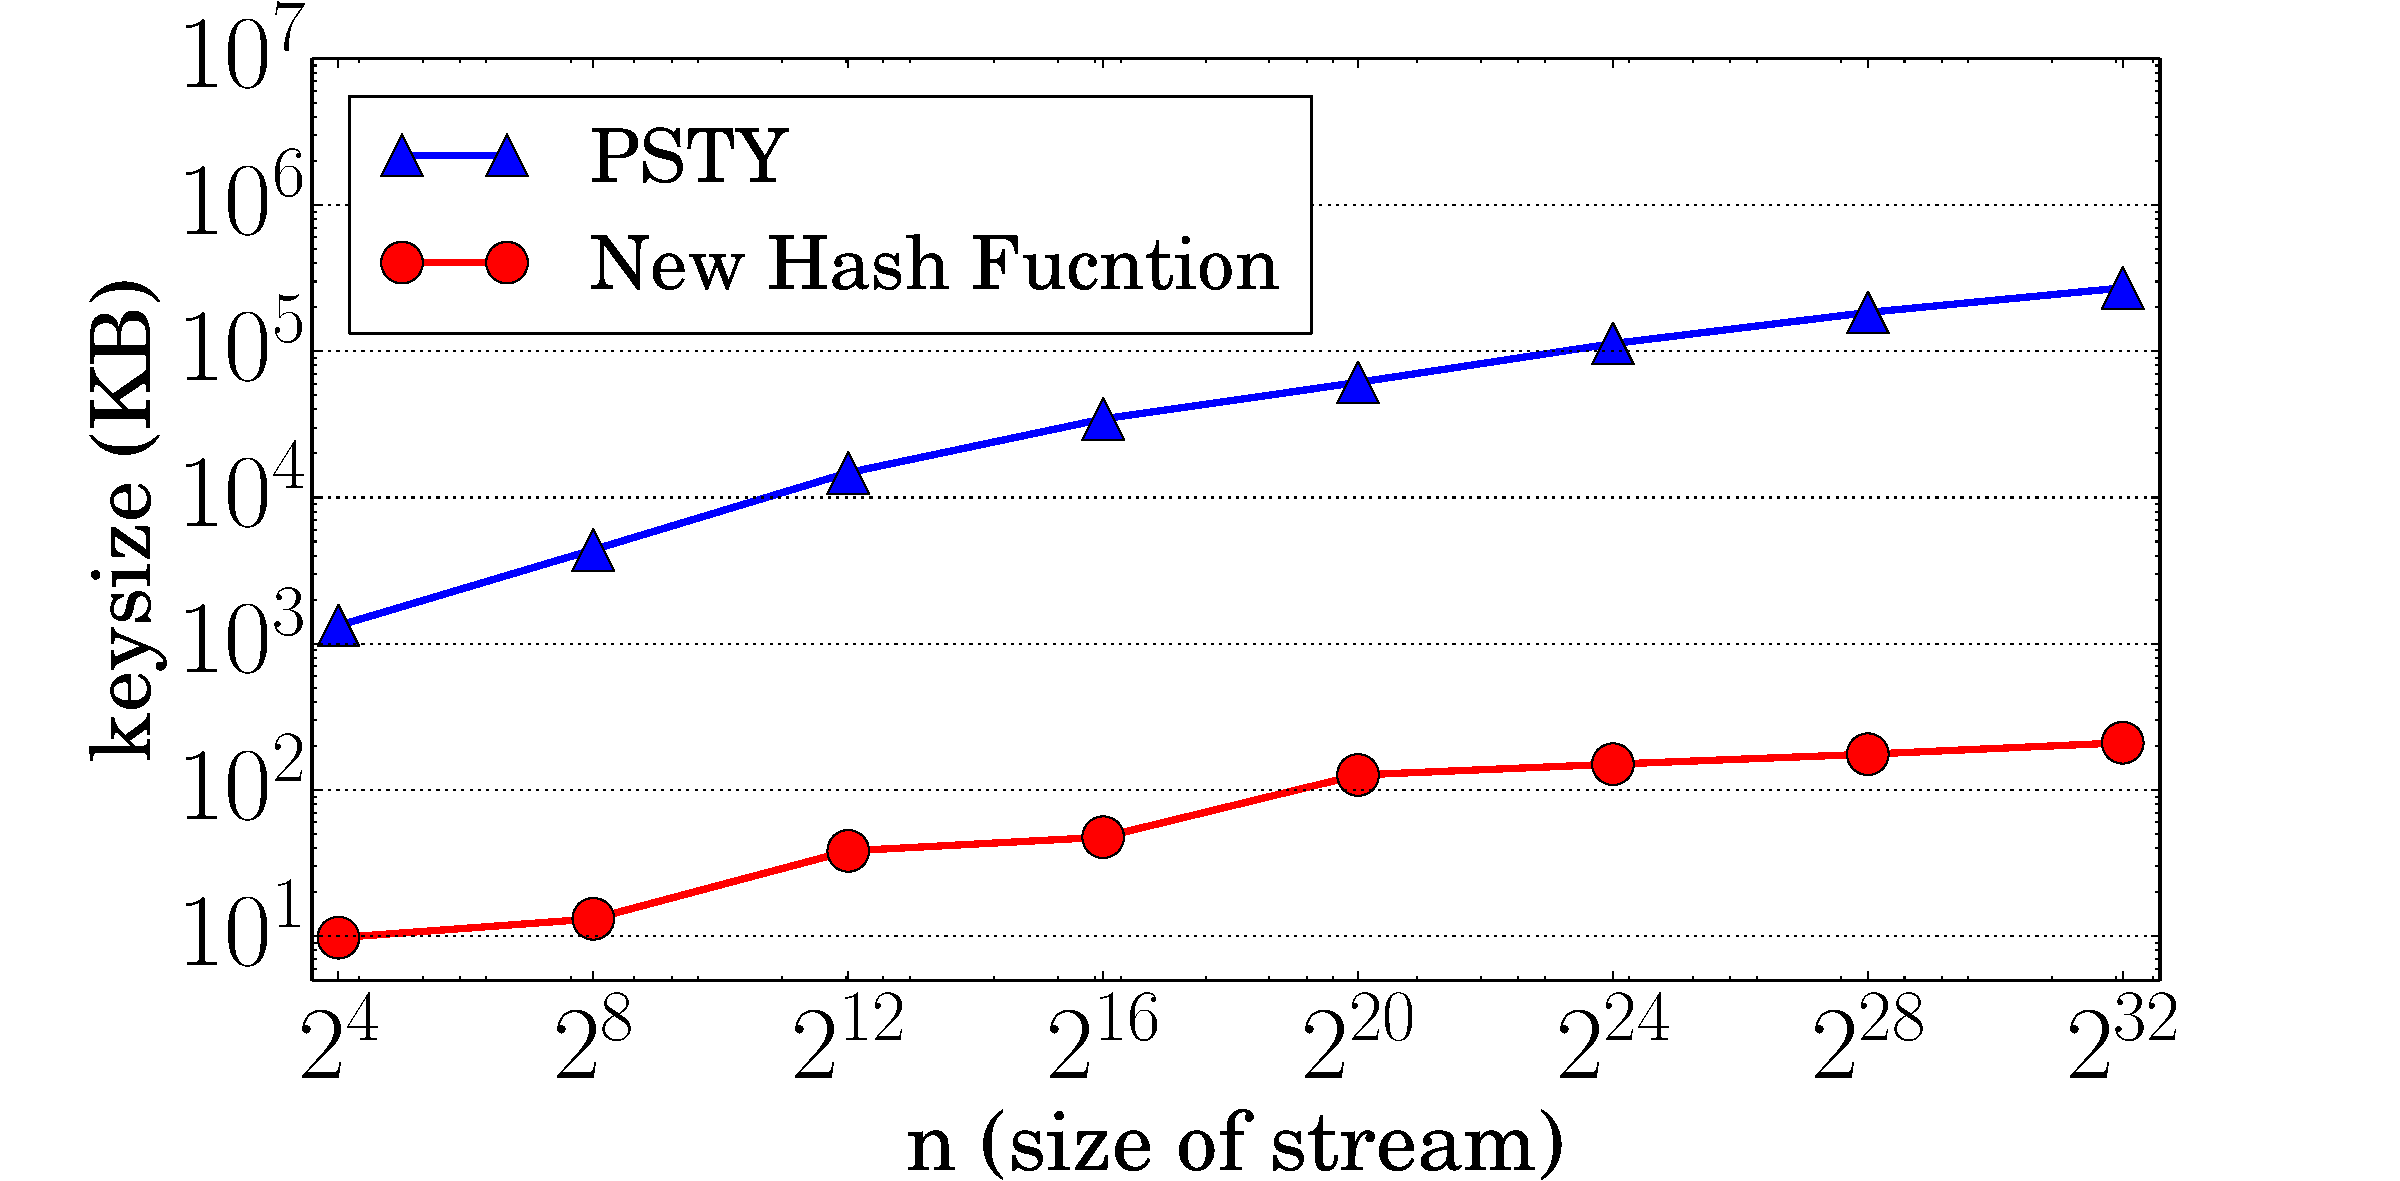
\includegraphics[scale = 0.23]{fig/keysize.pdf}
\caption{Key size of the hash functions. In the $x$ axis, we present the size $n$ of the stream and in the $y$ axis we show the key size in KB. The figure is in $\log-\log$ scale. The key size of $h_{new}$ is only 0.73\% when $n=2^4$, and 0.077\% when $n=2^{32}$, of $h_{old}$.}\label{keysize}
\end{minipage}\hfill
\end{figure*}

\section{Optimization}\label{modification}

%\babis{the algorithm is not correct, please change according to our discussions}
%\babis{For probability, use $\Pr[x=5]$}
In this section, we introduce a modified labeling function for the PSTY scheme~\cite{DBLP:conf/eurocrypt/PapamanthouSTY13} that reduces the space complexity by a factor of $\sqrt{n}$, except with negligible probability. Since this labeling function does not rely on any properties of the hash function, the modification also applies to any instantiations with the same projection function, inverse projection function and the $\gamma$ function introduced in section~\ref{instantiation}.

\ignore{
\begin{defn}[Modified Labeling]\label{modified_label}
Let $T_{\mathcal{C}}$ be a structured binary tree, where $\mathcal{C} = [c_{0}, c_{1}, \dots, c_{M-1}]$. For every node $w \in T_{\mathcal{C}}$ we define its label $\lambda(w) = \sum_{v\in \textsf{\emph{range}}(w)} c_v\cdot \delta_{w}(v) \bullet \textsf{\small \emph{rand()}}$, where $\delta_{w}(v)$ is the unit update defined by Definition~\ref{delta}, \textsf{\small \emph{rand()}} outputs a random vector from $\{-1,1\}^{k \cdot t}$ and $\bullet$ is the scalar dot product.
\end{defn}

}

\begin{defn}[Modified Labeling]\label{modified_label}
Let $T_{\mathcal{C}}$ be a structured binary tree, where $\mathcal{C} = [c_{0}, c_{1}, \dots, c_{M-1}]$. For every node $w \in T_{\mathcal{C}}$ we define its label $\lambda(w) = \sum_{v\in \textsf{\emph{range}}(w)} c_v\cdot \delta_{w}(v) \bullet \emph{\textsf{\small rand()}}$, where $\delta_{w}(v)$ is the unit update defined by Definition~\ref{delta}, $\emph{\textsf{\small rand()}}$ outputs a random bit from $\{-1,1\}$ and $\bullet$ is the scalar product.
\end{defn}

The random function \textsf{\small rand()} can be generated and retrieved by a pseudorandom generator with a public key. Given the $\gamma$ function as Equation~\ref{gamma1}, it is obvious that $\mathcal{L}_w(v) = c_v\cdot \delta_w(v)$. Next, we prove the size of the labels will be reduced to $O(\sqrt{n}) $ by this optimization.



\begin{lemma}\label{lemma_iid}
Assume elements in $\mathcal{C} = [c_{0}, c_{1}, \dots, c_{M-1}]$ are independent and identically distributed (i.i.d.), with mean $\mu$ and variance $\sigma^2$. For a node $w$ and a leaf $v\in\textsf{\emph{range}}(w)$, Let $\mathcal{P}_w(v)= c_{v} \cdot \delta_{w}(v) \bullet \textsf{\small \emph{rand()}} = [p_{1}, p_{2}, \dots, p_{{k \cdot t}}]$. Let $\delta_{w}(v) =[\delta_{1}, \delta_{2}, \dots, \delta_{k \cdot t}]$. For $1 \leq j \leq k \cdot t$, we have
\[  
  \{\begin{array}{l l}
    p_{j}=0 & \quad \text{if $\delta_{j}=0$;}\\
    p_{j} \emph{ is }i.i.d.\emph{ with mean 0 and variance } \mu^2+\sigma^2 & \quad \text{if $\delta_{j}=1$.}
  \end{array} 
  \]
\end{lemma}

\begin{proof}
For $1\le j\le k\cdot t$, $\delta_j$ is a deterministic binary value by Definition~\ref{delta}. In the first case, $p_{j}=0$ is trivially true when $\delta_{j}=0$. We consider the second case when $\delta_{j}=1$. Since \textsf{\small rand()} returns $1(-1)$ with $1/2$ probability independently and all elements in $\mathcal{C}$ are independent and identically distributed, we have the probability mass function of $p_{j}$ as the follows:
$$f_{p_j}(x)=
\begin{cases}
\frac{1}{2}f_{C}(x)& x>0\\
\frac{1}{2}f_{C}(-x)& x<0
\end{cases},$$
where $f_{C}$ is the probability mass function of elements in $C$. Since the distribution of $C$ has mean $\mu$ and variance $\sigma^{2}$, we have $\mu_{p_j} = 0$ and $\sigma_{p_j}^2 = \mu^2+\sigma^2$.
\end{proof}



\begin{lemma}\label{lemma_gaussian}
Let the label of the root $\lambda(r) =[\lambda_{1}, \lambda_{2}, \dots, \lambda_{k \cdot t}]$. For $1\le j\le k\cdot t$, let $n_j$ be the total number of leaves with nonzero $p_j$ defined in Lemma~\ref{lemma_iid}. Then, $\frac{\lambda_{j}}{\sqrt{n_{j}}}$ follows Gaussian distribution $N(0, \mu^2+\sigma^2)$ as $n_{j} \to \infty$.
\end{lemma}



\begin{proof}
Following directly from the Definition~\ref{modified_label} and Lemma~\ref{lemma_iid}, $\lambda_{j}$ is the summation of $n_{j}$ i.i.d random variables.  By the \textbf{Central Limit Theorem}, $\frac{\lambda_{j}}{\sqrt{n_{j}}} \sim N(0, \mu^2+\sigma^2)$ as $n_{j} \to \infty$. 


\end{proof}

\begin{lemma}\label{lemma_bound}
Let \textbf{\emph{X}} be a Gaussian distribution with mean 0 and variance $\sigma^2$, then $\Pr[\textbf{\emph{X}}>t] < \frac{1}{\sqrt{2\pi} \sigma t}e^{-\frac{t^2}{2\sigma^2}}$. 
\end{lemma}

\begin{proof}
By definition, $\Pr[\textbf{X}>t] = \int_{t}^{\infty} \frac{1}{\sqrt{2\pi} \sigma} e^{-\frac{x^2}{2\sigma^2}} dx$. We can bound the above expression by the following: $$\int_{t}^{\infty} \frac{1}{\sqrt{2\pi} \sigma} e^{-\frac{x^2}{2\sigma^2}} dx < \frac{1}{\sqrt{2\pi} \sigma t} \int_{t}^{\infty}xe^{-\frac{x^2}{2\sigma^2}} dx = \frac{1}{\sqrt{2\pi} \sigma t}e^{-\frac{t^2}{2\sigma^2}}$$. 
\end{proof}



\begin{theorem}
Let $w$ be any node in a generalized hash tree. Every element $\lambda_{j}$ of its modified labeling $\lambda(w)$ by Definition~\ref{modified_label} is in $[-t\sqrt{n}, t\sqrt{n}]$ for some constant $t$, except with negligible probability \textsf{\small \emph{neg($t$)}}.
\end{theorem}


\begin{proof}
By Lemma~\ref{lemma_gaussian}, $\frac{\lambda_{j}}{\sqrt{n_{j}}} \sim N(0, \mu^2+\sigma^2)$. Therefore,

\begingroup\makeatletter\def\f@size{9}\check@mathfonts
\def\maketag@@@#1{\hbox{\m@th\large\normalfont#1}}%
\begin{align*}
&\Pr[|\lambda_{j}| > t\sqrt{n}] < \Pr[|\lambda_{j}| > t\sqrt{n_{j}}] \nonumber \text{\ \ (Lemma~\ref{lemma_gaussian})}\\
&= \Pr[|\frac{\lambda_{j}}{\sqrt{n_{j}}}| > t] \\
&= 2\Pr[\frac{\lambda_{j}}{\sqrt{n_{j}}} > t] \\
&< 2\times \frac{1}{\sqrt{2\pi(\mu^2+\sigma^2)}  t}e^{-\frac{t^2}{2(\mu^2+\sigma^2)}} \nonumber \text{\ \ (Lemma~\ref{lemma_bound})},
\end{align*}\endgroup
which is negligible \textsf{\small{neg($t$)}}.

\end{proof}


\section{Experiments and Comparisons}\label{experiments}

\begin{figure*}[Ht!]
\centering
\begin{minipage}[t]{.49\textwidth}
\centering
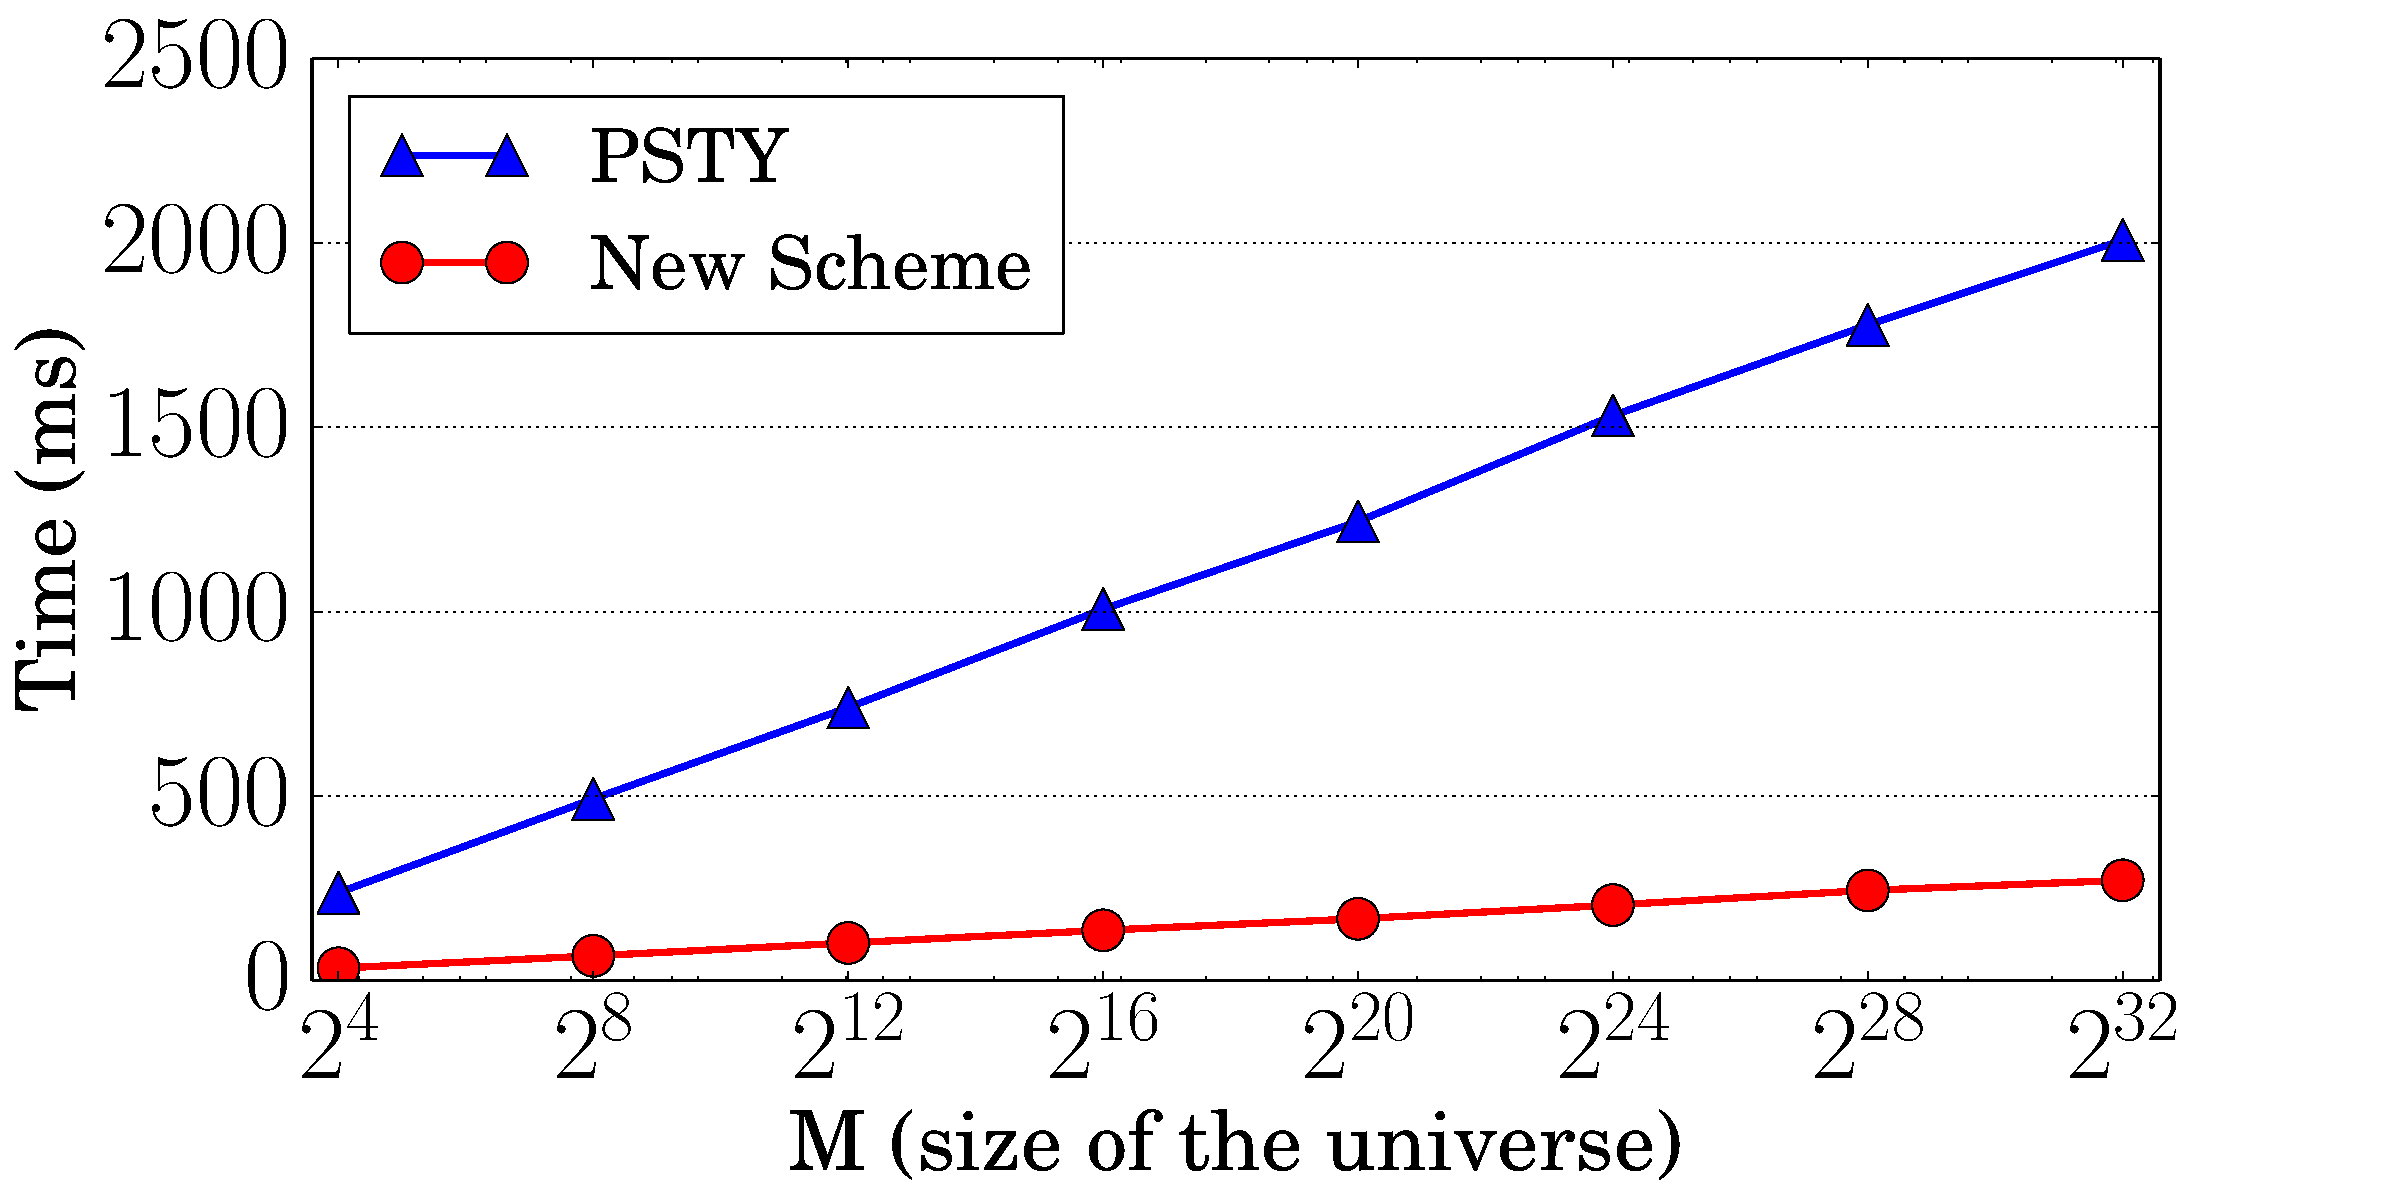
\includegraphics[scale = 0.23]{fig/verifytime_1.pdf}
\caption{Verification time. The $x$ axis is the size of universe $|M|$ in $\log$ scale. The size of stream is fixed to $n = 2^{32}$. The new scheme with $h_{new}$ achieves $7.5\times$ speed up.}\label{verify_time}
\end{minipage}\hfill
\begin{minipage}[t]{.49\textwidth}
\centering
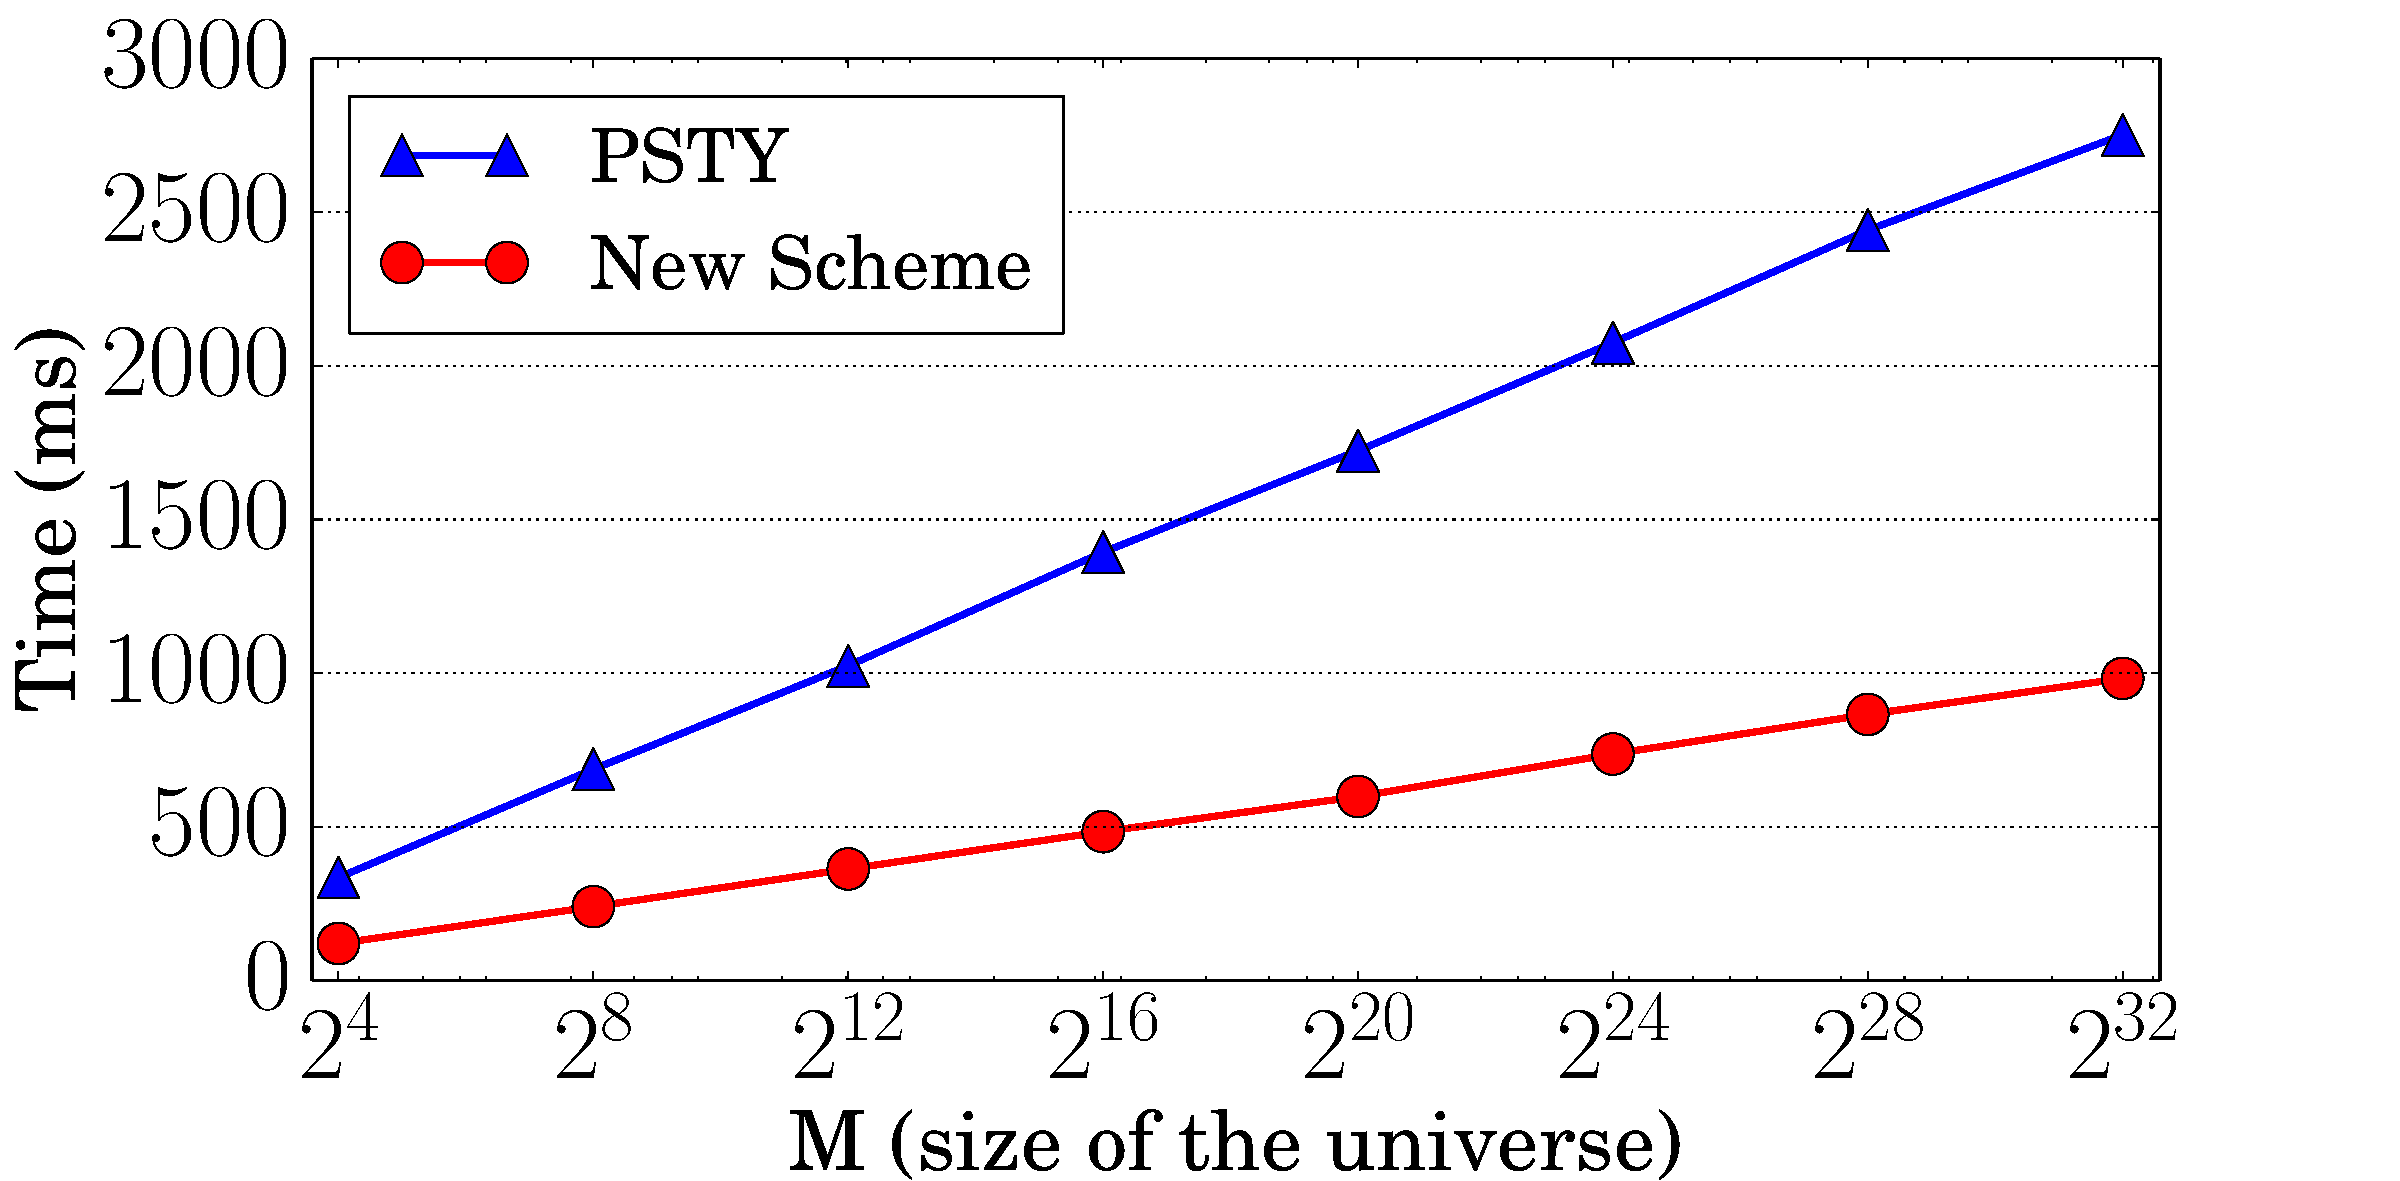
\includegraphics[scale = 0.23]{fig/updatetime_1.pdf}
\caption{Update time (client side).  The $x$ axis is the size of universe $|M|$ in $\log$ scale. The size of stream is fixed to $n = 2^{32}$. The new scheme with $h_{new}$ achieves $2.8\times$ speed up.}\label{update_time}
\end{minipage}\hfill
\end{figure*}


We implement the instantiations of our abstract SADS with both the hash function $h_{old}$ in PSTY~\cite{DBLP:conf/eurocrypt/PapamanthouSTY13} and our new GCK based hash function $h_{new}$ introduced in Section~\ref{new_hash}. We conduct a series of comparing experiments of these two instantiations. We show major performance improvements due to the GCK hash function.
\ignore{
First, we compare the performance of $h_{old}$ and $h_{new}$ in terms of the running time and key size. Next, we discuss the experimental results on all $6$ algorithms of Figure~\ref{algorithms_sads} by both instantiations. In particular, we present the empirical performance of \emph{verification}, \emph{update} and \emph{range search query} by the two instantiations.  }

{First, we highlight the asymptotic improvement of $h_{new}$ compared to $h_{old}$ in terms of the running time and key size. Next, we discuss the experimental results on various algorithms of Figure~\ref{algorithms_sads} for both instantiations. In particular, we present the empirical performance of \emph{verification}, \emph{update} and \emph{range search query} by the two instantiations.}


\vspace{1.5mm}\noindent{\bf Experiment setup.} The two instantiations are implemented in Mathlab 2014Ra and executed on a Windows 8.1 Desktop with 16GB of RAM.  The same data samples randomly generated are used in all experiments. We collected 10 runs for each data point and report the average.

There are two critical parameters involved in the experiments: 
\begin{enumerate}
\item The size of the stream $n$. This determines the parameter configuration of our GCK hash function $h_{new}$ by Algorithm~\ref{config_alg}. In particular, the running time and the key size of both $h_{new}$ and $h_{old}$ increase with respect to $n$. 
\item The size of the universe $M$. $|M|$ determines the size of the generalized hash tree (the generalized hash tree has $\log M$ layers), and consequently affects the running time of the query, update and verification of the SADS.
\end{enumerate}

\begin{table}[h!]\centering
%\caption{Detail statistics for $n=2^{32}$ and $|M| = 2^{32}$.}\label{asymptotic}
\caption{Asymptotic comparison between $h_{old}$ and $h_{new}$. Notice $t = \nu \log q$.}\label{asymptotic}
\begin{tabular}{|c|c|c|}

\hline
{}&running time&key size\\
\hline
PSTY&$O(\nu^2\log q)$&$O(\nu^2\log q)$\\
\hline
New Hash Function&$O(k\log k\log p)$&$O(k\log p)$\\
\hline

\end{tabular}
\end{table}


{
\vspace{1.5mm}\noindent{\bf Asymptotic comparison.} Table~\ref{asymptotic} shows the asymptotic complexity comparison of running time of hash functions and key size between $h_{old}$ and $h_{new}$\footnote{PSTY~\cite{DBLP:conf/eurocrypt/PapamanthouSTY13} has a set of different notations for parameters.}. As it is shown in both Section~\ref{instantiation} and PSTY~\cite{DBLP:conf/eurocrypt/PapamanthouSTY13}, the hash function $h_{old}$ is a matrix--vector multiplication, of which the running time is $O(\nu^2\log q)$ and the key size is the size of the matrix, $O(\nu^2\log q)$. The hash function $h_{new}$ constructed in Section~\ref{gck} is primarily based on polynomial multiplication, of which the running time using FFT is $O(k\log k\log p)$ and the key size is $O(k\log p)$. 

We generate parameters (e.g. $k$, $p$ and $q$) according to the size of the stream $n$ to ensure approximately the same security parameter ($100^+$ in both cases). In practice, $k$ is much smaller than $\nu$ and $\log p$ is roughly equal to $\log q$. Consequently, the improvement is rather significant.

\vspace{1.5mm}\noindent{\bf Running time of the hash functions.} Figure~\ref{hashtime} shows the running time of hashing one message by both $h_{old}$ and $h_{new}$ with increasing $n$. Our new hash function $h_{new}$ turns to outperform $h_{old}$ by orders of magnitude. Specifically, $h_{new}$ runs $1.6 \times$ faster when $n = 2^4$, and $9.8\times$ faster when $n = 2^{32}$, than $h_{old}$. This matches the asymptotic complexity comparison mentioned above. More importantly, the time cost of $h_{new}$ doesn't grow much as $n$ increases while it grows quasi-linearly with $n$ for $h_{old}$. As a result, the new hash function $h_{new}$ supports much larger streaming volume than $h_{old}$. 
%\babis{I want to cry with $h_{old}$ and $h_{new}$, PLEASE FIX THE NOTATION}

\begin{figure*}[Ht!]
\centering
\begin{minipage}[t]{.49\textwidth}
\centering
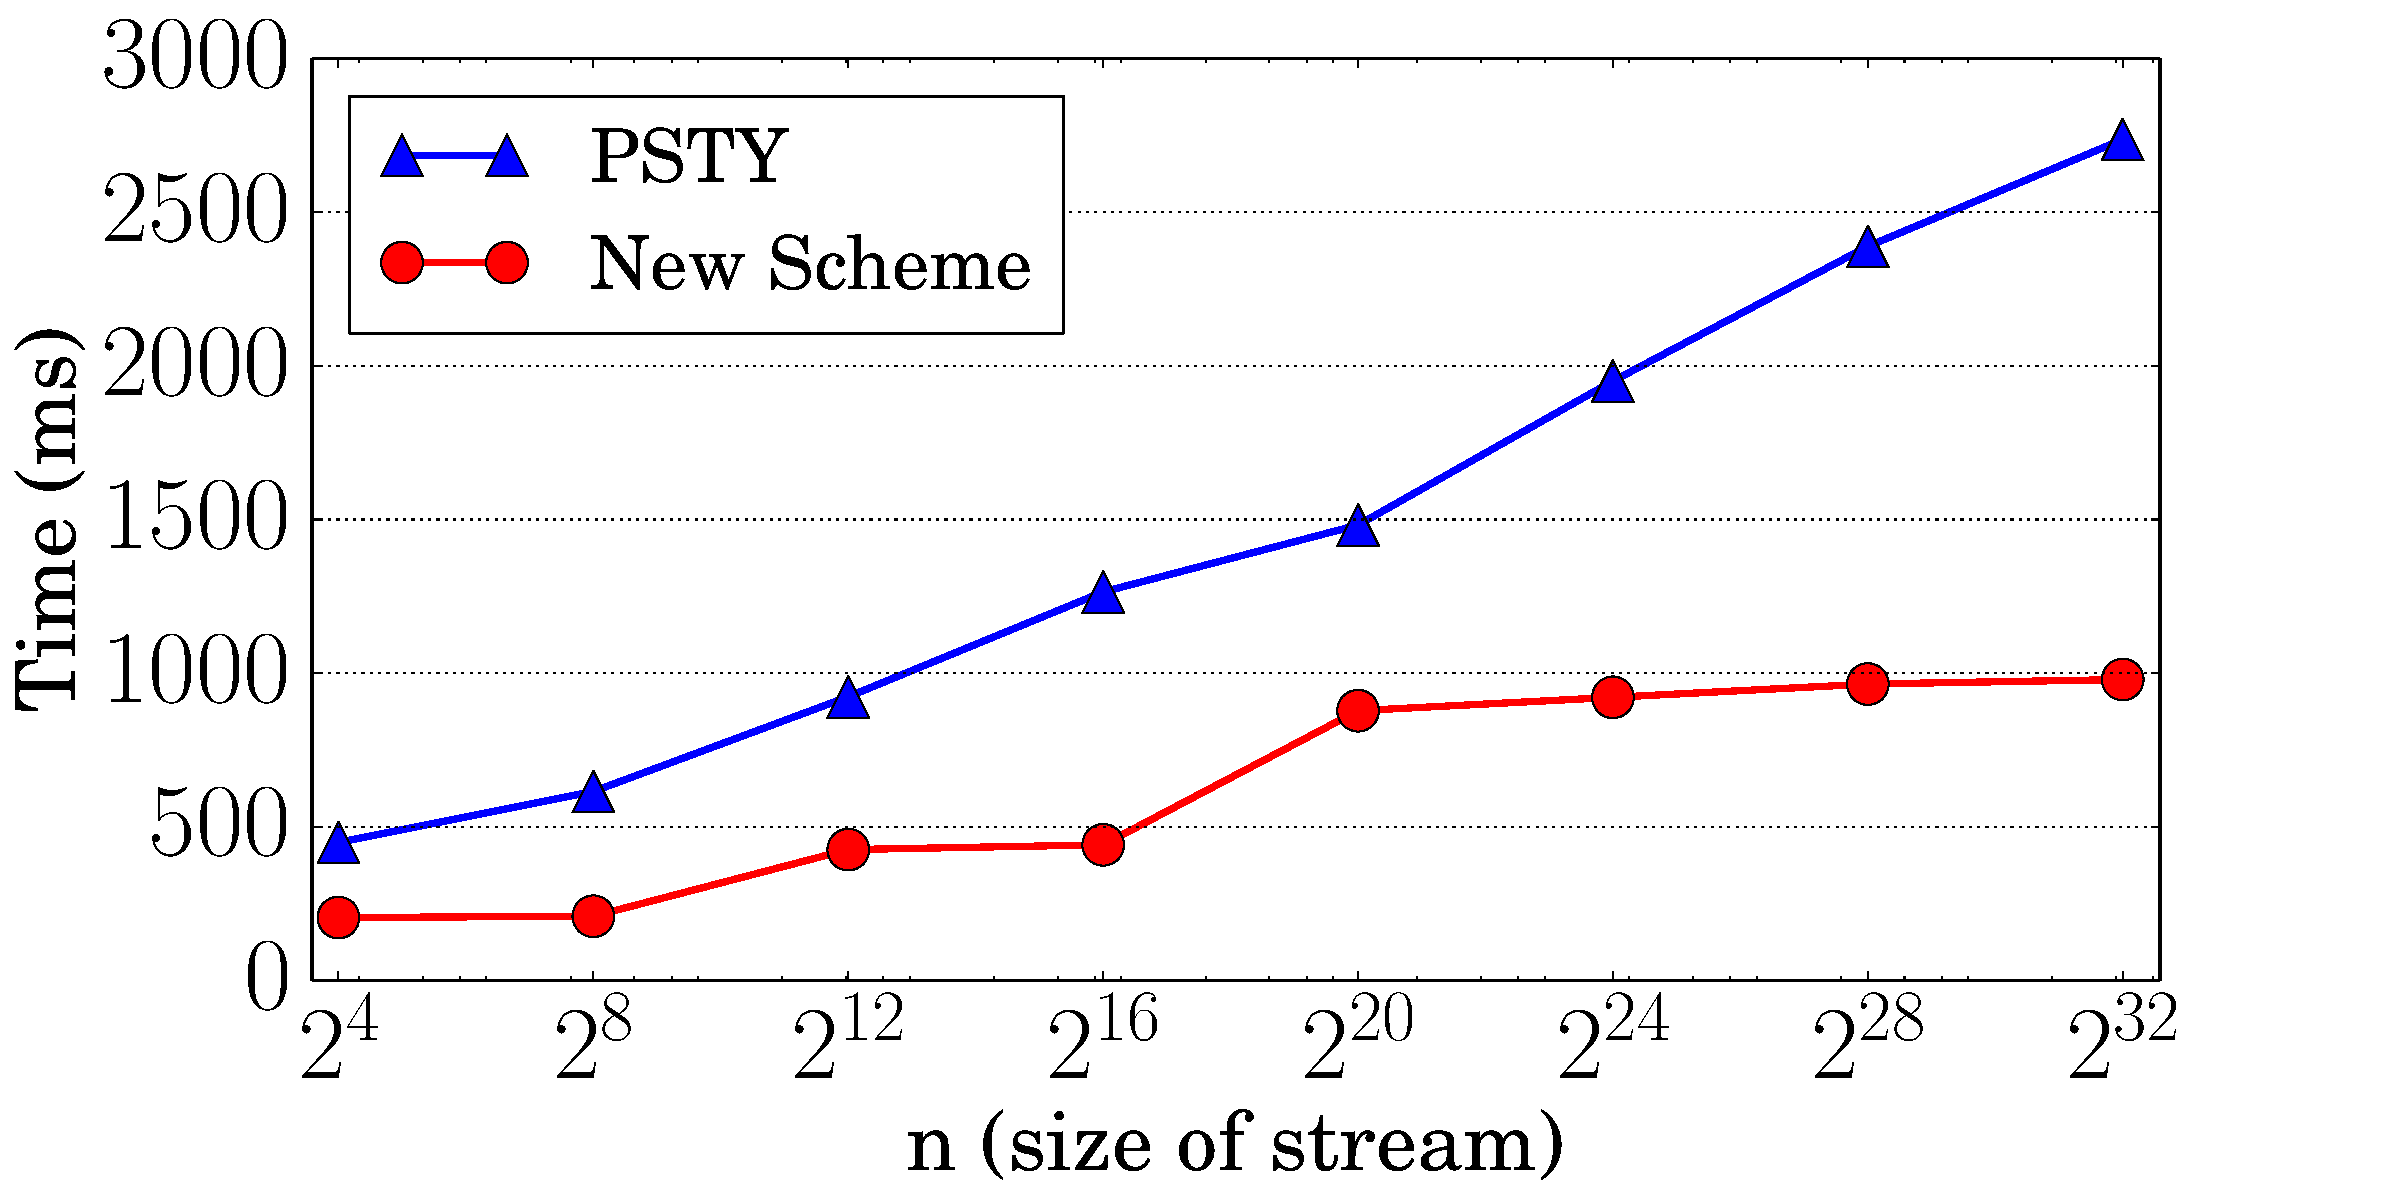
\includegraphics[scale = 0.23]{fig/updatetime_2.pdf}
\caption{Update time (client side). The $x$ axis is the size of stream $n$ in $\log$ scale. The size of the universe is fixed to $|M| = 2^{32}$. The new scheme with $h_{new}$ is $1.7\times$ faster when $n=2^4$, and $3.0\times$ faster when $n=2^{32}$, than the scheme with $h_{old}$.}\label{update_time2}
\end{minipage}\hfill
\begin{minipage}[t]{.49\textwidth}
\centering
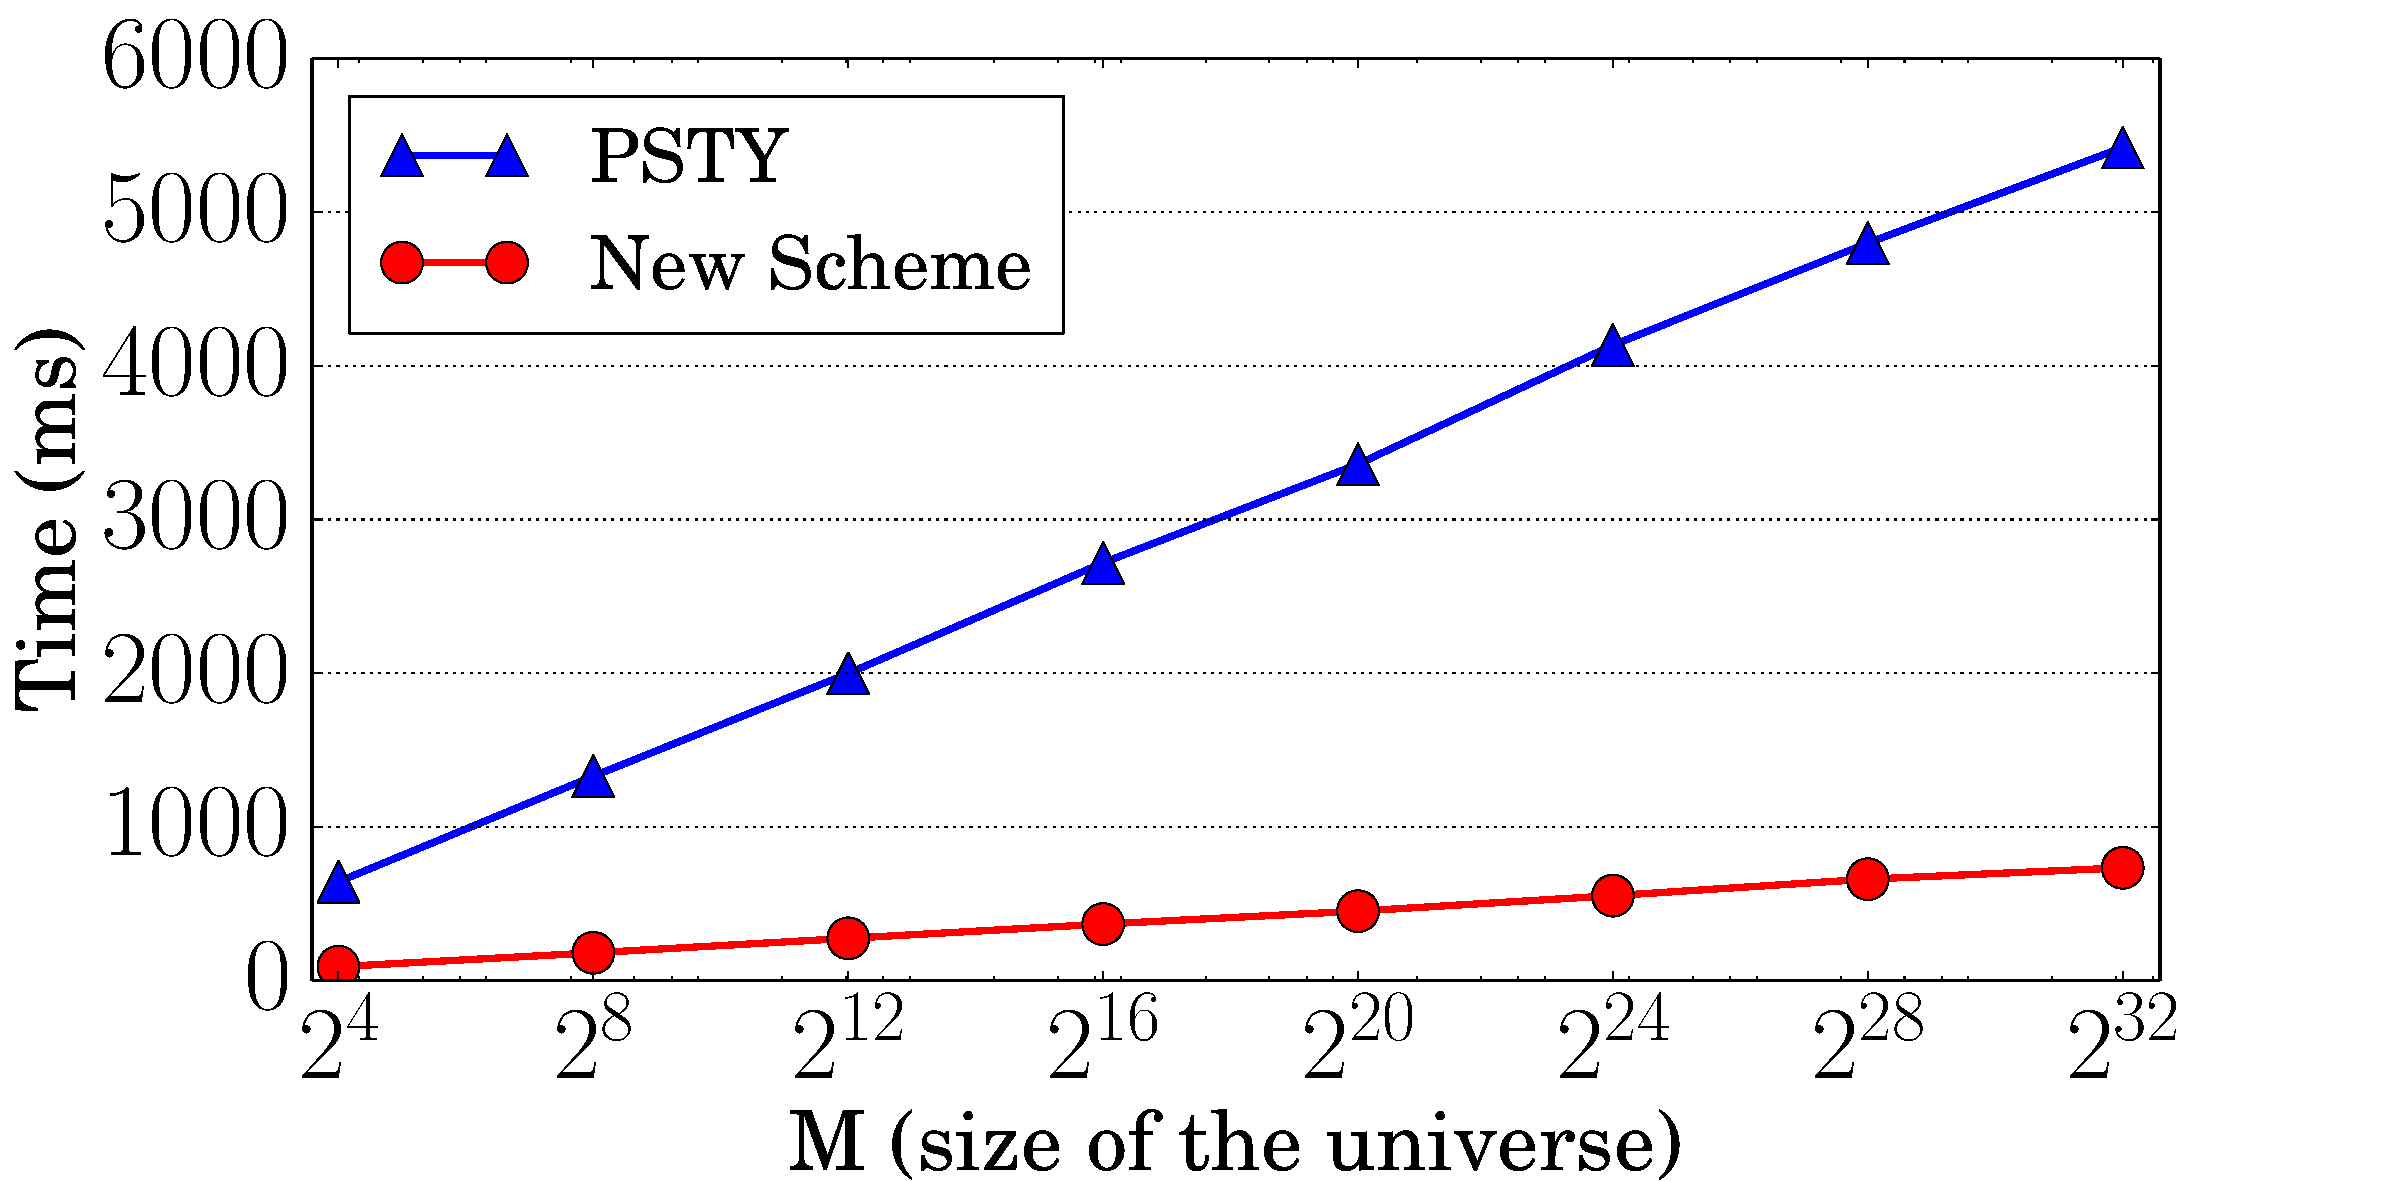
\includegraphics[scale = 0.23]{fig/range_search_1.pdf}
\caption{Range search time. The $x$ axis is the size of universe $|M|$ in $\log$ scale. The size of stream is fixed to $n = 2^{32}$. The new scheme with $h_{new}$ achieves $7.4\times$ speed up.}\label{range_time}
\end{minipage}\hfill
\end{figure*}


\vspace{1.5mm}\noindent{\bf Key size of hash functions.} Figure~\ref{keysize} shows the key sizes of both $h_{old}$ and $h_{new}$ with increasing $n$, which is plotted in $\log$-$\log$ scale. The key size of our new hash $h_{new}$ is only $0.73\%$ of the one of $h_{old}$ when $n = 2^4$, and $0.077\%$ of the ones of $h_{old}$ when $n = 2^{32}$. This significant improvement is due to the advantages of circular lattices over regular lattices. Moreover, the key size of $h_{new}$ grows roughly linearly with $n$ while it grows quadratically with $n$ for $h_{old}$. Notice the public key of the abstract SADS is the key of the two hash functions ${\bf {\cal H}_{L}}$, ${\bf {\cal H}_{R}}$. Hence, the improvement of hash function key size in Figure~\ref{keysize} applies directly to the public key size of the entire scheme.%\babis{the last two statements are not clear}
}

\vspace{1.5mm}\noindent{\bf Preprocessing.} In algorithms $\mathsf{initialize}()$ of Figure~\ref{algorithms_sads}, the digest and every node labels of the generalized hash tree are initialized to be $\bf 0$s. Hence, the preprocessing time is independent of the hash function choice.
Notice that in our implementations, the generalized hash tree is dynamically allocated, and the storage cost is proportional to the nonzero values stored in the leaves. In this way, we can run the experiments on a large universe of size up to $|M| = 2^{32}$.

\vspace{1.5mm}\noindent{\bf Proof Computation.} The server needs to compute the result along with a proof, responding to a query from the verifier. We discuss two ways to compute the proof on the server side. (1) The server constructs and stores the whole generalized hash tree, and returns the corresponding labels of nodes required by the proof. (2) The server only stores the values in the leaves of the generalized hash tree, and computes labels of nodes for a proof each time. There is a time-space trade-off between these two approaches. We choose the former in our implementations, in which case the proof computation is just an index searching and returning procedure. Hence, the proof computation time is the same for both instantiations. 

\vspace{1.5mm}\noindent{\bf Verification.} Figure~\ref{verify_time} shows the comparison for verification time by the instantiation with $h_{new}$ and the instantiation with $h_{old}$. The $x$ axis is the size of the universe $M$. The upper bound of the streaming $n$ is fixed to $2^{32}$. As we can see, the instantiation with our new hash function $h_{new}$ outperforms the instantiation with $h_{old}$ dramatically. Specifically, the verification time of the new instantiation with $h_{new}$ is 7.5 times faster than the one with $h_{old}$. Moreover, Figure~\ref{verify_time} shows that the verification time grows on the order of $O(\log M)$, matching what the algorithm $\mathsf{verify}()$ indicates. Finally, the verification time is only $10\sim100$ milliseconds with $h_{new}$, which makes the new scheme practical.


\vspace{1.5mm}\noindent{\bf Update.} Figure~\ref{update_time} shows that the instantiation with $h_{new}$ runs 2.8 times faster than the one with $h_{old}$ for the client side update. Notice that the client side update and the server side update go through the same computations, except that the server also updates the labels of nodes along the verification path. Therefore, the time cost of the client side update and the server side update is roughly the same. We omit the comparison for the server update time here. Moreover, the update time grows logarithmically with $M$ as desired in Figure~\ref{update_time}.

In practice, the size of the universe $|M|$ is usually fixed for a certain streaming application. To illustrate such scenario, we show the update time as $n$ increases, with $|M|$ fixed to $2^{32}$. Figure~\ref{update_time2} shows that the instantiation with $h_{new}$ is $1.7\sim3.0$ times faster than the one with $h_{old}$. The larger streaming volume $n$ results in the more significant improvement in terms of update time.



\vspace{1.5mm}\noindent{\bf Range search.} The range search functionality is implemented and the results are shown in Figure~\ref{range_time}. The range search time cost of both instantiations is slightly larger than two times of their verification time cost, and hence grows logarithmically with $M$ as desired.
Moreover, the range search of the instantiation with $h_{new}$ is 7.4 times faster than the one with $h_{old}$.

\begin{table}[h!]\small
\caption{Detail statistics for $n=2^{32}$ and $|M| = 2^{32}$.}\label{data}
\begin{tabularx}{0.48\textwidth}{p{1.2cm}|c|c|c|c|c}
%\begin{tabular}{|c|c|p{0.9cm}|p{1.2cm}|p{0.6cm}|p{0.9cm}|}
%\begin{tabular}{|c|c|c|c|c p{0.6cm}|c|}
\hline
{}&running&key size&verification&update&range\\
%\hline
{}&time (ms)&(MB)&(s)&(s)&search (s)\\
\hline
Instantiation&\multirow{2}{*}{2.74}&\multirow{2}{*}{0.21}&\multirow{2}{*}{0.27}&\multirow{2}{*}{0.98}&\multirow{2}{*}{0.73}\\
with $h_{new}$&&&&&\\
\hline
Instantiation&\multirow{2}{*}{26.84}&\multirow{2}{*}{265.02}&\multirow{2}{*}{2.01}&\multirow{2}{*}{2.75}&\multirow{2}{*}{5.42}\\
with $h_{old}$&&&&&\\
\hline

\end{tabularx}
\end{table}

%\yi{Please update the caption/legend in the figures accordingly. Use instantiation with $h_{new}$ and instantiation with $h_{old}$ .}

Finally, Table~\ref{data} shows the statistics for both instantiations when $n=2^{32}$ and $|M|=2^{32}$. We can see that hashing a message by $h_{new}$ only takes 2.74 milliseconds while \emph{update}, \emph{verification} and \emph{range search} of the new instantiation with $h_{new}$ all takes less than one second. Meanwhile, the key size of the new scheme is only 0.21MB, which is practical to store and manage, to the key of $h_{old}$ which is 265MB.


\section{Conclusion}\label{conclusion}
This paper proposes an abstract construction of a streaming authenticated data structure, and presents two instantiations of the proposed abstraction. The first intantiation is the PSTY work~\cite{DBLP:conf/eurocrypt/PapamanthouSTY13}. The second instantiation is a scheme with a different collision-resistant hash function, which is based on the generalized compact knapsack (GCK) problem~\cite{GCK}. The new hash function is carefully parameterized, such that it is secure against state-of-the-art attacks~\cite{wagner02,lattice}. 

We implement both schemes. Our experiments highlight major savings in prover complexity and public key size of our second (new) instantiation over the PSTY work.
\section*{Acknowledgments} We thank Bobby Bhattacharjee, Youngsam Park, Elaine Shi and Emil Stefanov for many useful discussions. 

This paper is dedicated to Emil's memory, who encouraged us to investigate the practicality of the PSTY paper.
%\bibliographystyle{abbrv}
%\bibliography{babis,refs,yupeng,yi}
\input{reference.bbl}
%\balancecolumns
% That's all folks!
\end{document}
